% Created 2024-05-03 Παρ 18:21
% Intended LaTeX compiler: pdflatex
\documentclass[11pt]{report}
\usepackage[utf8]{inputenc}
\usepackage[T1]{fontenc}
\usepackage{graphicx}
\usepackage{longtable}
\usepackage{wrapfig}
\usepackage{rotating}
\usepackage[normalem]{ulem}
\usepackage{amsmath}
\usepackage{amssymb}
\usepackage{capt-of}
\usepackage{hyperref}
\usepackage{booktabs}
\usepackage{import}
\usepackage[LGR, T1]{fontenc}
\usepackage[greek, english, american]{babel}
\usepackage{alphabeta}
\usepackage{esint}
\usepackage{mathtools}
\usepackage{esdiff}
\usepackage{makeidx}
\usepackage[acronym]{glossaries}
\usepackage{newfloat}
\usepackage{minted}
\usepackage[a4paper, margin=3cm]{geometry}
\usepackage{chemfig}
\usepackage{svg}
\usepackage[automake]{glossaries-extra}
\usepackage{fancyhdr}
\geometry{a4paper,width=150mm,top=25mm,bottom=25mm}
\makeglossaries
\newcommand{\HRule}{\rule{\linewidth}{0.5mm}}
\date{}
\title{ΒΙΟΑΠΟΔΟΜΗΣΗ ΥΠΟΛΕΙΜΜΑΤΩΝ ΤΡΟΦΙΜΩΝ ΚΑΙ ΠΑΡΑΓΩΓΗ ΒΙΟΑΕΡΙΟΥ ΜΕΣΩ ΑΝΑΕΡΟΒΙΑΣ ΧΩΝΕΥΣΗΣ ΣΕ ΕΡΓΑΣΤΗΡΙΑΚΗ ΚΑΙ ΠΙΛΟΤΙΚΗ ΚΛΙΜΑΚΑ Προβλήματα στην αναερόβια χώνευση Μεθόδοι Επεξεργασίας}
\hypersetup{
 pdfauthor={Βιδιάνος Γιαννίτσης},
 pdftitle={ΒΙΟΑΠΟΔΟΜΗΣΗ ΥΠΟΛΕΙΜΜΑΤΩΝ ΤΡΟΦΙΜΩΝ ΚΑΙ ΠΑΡΑΓΩΓΗ ΒΙΟΑΕΡΙΟΥ ΜΕΣΩ ΑΝΑΕΡΟΒΙΑΣ ΧΩΝΕΥΣΗΣ ΣΕ ΕΡΓΑΣΤΗΡΙΑΚΗ ΚΑΙ ΠΙΛΟΤΙΚΗ ΚΛΙΜΑΚΑ Προβλήματα στην αναερόβια χώνευση Μεθόδοι Επεξεργασίας},
 pdfkeywords={},
 pdfsubject={},
 pdfcreator={Emacs 29.3 (Org mode 9.6.15)}, 
 pdflang={English}}
\makeatletter
\newcommand{\citeprocitem}[2]{\hyper@linkstart{cite}{citeproc_bib_item_#1}#2\hyper@linkend}
\makeatother

\usepackage[notquote]{hanging}
\begin{document}

\renewcommand{\abstractname}{Περίληψη}
\renewcommand{\tablename}{Πίνακας}
\renewcommand{\figurename}{Σχήμα}
\renewcommand{\chaptername}{Κεφάλαιο}
\renewcommand{\chapterautorefname}{Κεφάλαιο}
\renewcommand{\partname}{Μέρος}
\renewcommand{\listfigurename}{Περιεχόμενα Διαγραμμάτων: }
\renewcommand{\listtablename}{Περιεχόμενα Πινάκων: }
\renewcommand\listingscaption{Κώδικας}
\pagestyle{fancy}
\fancyhead{}
\fancyhead[L]{\chaptername~\thechapter}
\fancyhead[R]{Βιδιάνος Γιαννίτσης}
\newacronym{fw}{ΥΤ}{υπολείμματα τροφών}
\newacronym{fao}{FAO}{Οργανισμός Τροφίμων και Αγρονομίας των Ηνωμένων Πολιτειών}
\newacronym{co2eq}{$CO_2$-eq}{ισοδύναμο διοξειδίου του άνθρακα}
\newacronym{xyta}{ΧΥΤΑ}{Χώρους Υγειονομικής Ταφής Απορριμάτων}
\newacronym{syngas}{syngas}{αέριο σύνθεσης}
\newacronym{pla}{PLA}{πολυγαλακτικό οξύ}
\newacronym{trl}{TRL}{technology readiness level}
\newacronym{vfa}{VFAs}{πτητικά λιπαρά οξέα}
\newacronym{hrt}{HRT}{υδραυλικός χρόνος παραμονής}
\newacronym{olr}{OLR}{ρυθμός οργανικής φόρτισης}
\newacronym{uasb}{UASB}{αντιδραστήρας ανοδικής ροής διαμέσου στρώσης ιλύος}
\newacronym{mix}{μιξ}{σκεύασμα ενζύμων και μικροοργανισμών}
\newacronym{ad}{ΑΧ}{αναερόβια χώνευση}
\newacronym{ts}{TS}{ολικά στερεά}
\newacronym{vs}{VS}{πτητικά στερεά}
\newacronym{cod}{COD}{χημικά απαιτούμενο οξυγόνο}
\newacronym{scod}{sCOD}{διαλυτό COD}
\newacronym{tcod}{tCOD}{ολικό COD}
\newacronym{pi}{PI}{Process Intensification}
\newacronym{ssf}{SSF}{Solid State Fermentation}

\renewcommand{\contentsname}{Κεφάλαια: }
\begin{titlepage}

\begin{center}
  \begin{minipage}{0.2\textwidth}
    \begin{flushleft}
      \includegraphics[width=1\textwidth]{~/Pictures/ntua_logo.png}\\[0.4cm]    
    \end{flushleft}
  \end{minipage}
  \begin{minipage}{0.75\textwidth}
    \textsc{\bfseries \Large ΕΘΝΙΚΟ ΜΕΤΣΟΒΙΟ ΠΟΛΥΤΕΧΝΕΙΟ}\\[0.2cm]
    \textsc{\bfseries \Large ΣΧΟΛΗ ΧΗΜΙΚΩΝ ΜΗΧΑΝΙΚΩΝ}\\[0.2cm]
    \textsc{\large \bfseries ΤΟΜΕΑΣ IV: ΣΥΝΘΕΣΗ ΚΑΙ ΑΝΑΠΤΥΞΗ ΒΙΟΜΗΧΑΝΙΚΩΝ ΔΙΑΔΙΚΑΣΙΩΝ}\\[0.2cm]
    \textsc{\bfseries \large ΕΡΓΑΣΤΗΡΙΟ ΟΡΓΑΝΙΚΗΣ ΧΗΜΙΚΗΣ \\ ΤΕΧΝΟΛΟΓΙΑΣ}\\[0.2cm]
  \end{minipage}
  \\[2.5cm]

  \HRule \\[0.3cm]
  \Huge Βιοαποδόμηση Υπολειμμάτων Τροφίμων και Παραγωγή Βιοαερίου μέσω Αναερόβιας Χώνευσης σε Εργαστηριακή και Πιλοτική Κλίμακα\\[2.5cm]

  \huge Διπλωματική Εργασία \\[0.3cm]
   \begin{minipage}{0.4\textwidth}
    \begin{flushleft}
      \emph{\LARGE Συγγραφέας:}\\
	\emph{\LARGE Αριθμός Μητρώου:} \\
	\emph{\LARGE e-mail:}
      \end{flushleft}
    \end{minipage}
    \begin{minipage}{0.4\textwidth}
      \begin{flushright} \large
	\LARGE Βιδιάνος Γιαννίτσης\\
	\LARGE ch19113\\
	\LARGE vidianosgiannitsis@gmail.com
      \end{flushright}
    \end{minipage}
    \HRule \\[0.3cm]
  \vfill
{\LARGE Αθήνα, 2024}

\end{center}

\end{titlepage}

\part*{Περιεχόμενα}
\label{sec:org3cf1203}
\tableofcontents
\pagebreak

\listoffigures
\pagebreak

\listoftables
\pagebreak

\printglossary
\printglossary[type = \acronymtype, title = Συντομογραφίες]

\part{Θεωρητικό Μέρος}
\label{sec:org7a25d26}
\chapter{Εισαγωγή}
\label{sec:org918ad29}

Τα \acrfull{fw} αποτελούν ένα σημαντικό πρόβλημα στις σύγχρονες κοινωνίες. Ο \acrfull{fao} υπολογίζει πως περίπου το 1/3 της παγκόσμιας παραγωγής τροφών ετησίως (1.3 δις τόνοι) χάνεται κατά την παραγωγική διαδικασία ή απορρίπτεται (\citeprocitem{14}{Ishangulyyev, Kim, and Lee 2019}).

Η μη ορθή διαχείριση των αποβλήτων αυτών επιβαρύνει κάθε έναν από τους τρείς πυλώνες της βιωσιμότητας. Συγκεκριμένα, έχει προσδιοριστεί πως το \acrfull{co2eq} που παράγεται λόγω της μη ορθής αυτής διαχείρισης των υπολείμματων ανέρχεται στους 3.3 δις τόνους (\citeprocitem{39}{Taheri et al. 2021}) . Ακόμη, έχει βρεθεί πως τα υπολείμματα τροφών που οφείλονται μόνο στην απόρριψη τροφών από καταναλωτές σε ανεπτυγμένες χώρες είναι σχεδόν όσα παράγουν οι υπό σακχάριες και αφρικανικές χώρες συνολικά (περίπου 230 εκατομμύρια) (\citeprocitem{14}{Ishangulyyev, Kim, and Lee 2019}). Οπότε η αποφυγή της δημιουργίας τόσων υπολειμμάτων - ή η καλύτερη αξιοποίηση τους - θα μπορούσε να λύσει πολλά προβλήματα υποσιτισμού. Ακόμη και στον οικονομικό τομέα, δημιουργούνται σοβαρά προβλήματα από την ανεξέλεγκτη αυτή απόρριψη καθώς η καθαρή αξία των τροφών που χάνονται ή απορρίπτονται σε κάποιο σημείο της εφοδιαστικής αλυσίδας είναι 936 δις δολλάρια ανά έτος με ελάχιστο κέρδος, καθώς πολύ μικρές ποσότητες των υπολειμμάτων αυτών αξιοποιούνται (\citeprocitem{14}{Ishangulyyev, Kim, and Lee 2019}) .

Μία από τις βασικότερες υποκατηγορίες \acrshort{fw} είναι τα οικιακά \acrshort{fw}. Αποτελούν το μεγαλύτερο κομμάτι της παγκόσμιας παραγωγής \acrshort{fw} αποτελώντας περίπου το \(61 \%\) αυτής (\citeprocitem{37}{“Statista - The Statistics Portal” n.d.}) . Στο \figurename \ref{fig:orgd4b1d00} φαίνεται η παγκόσμια παραγωγή \acrshort{fw} ανά τομέα.
\begin{figure}[htbp]
\centering
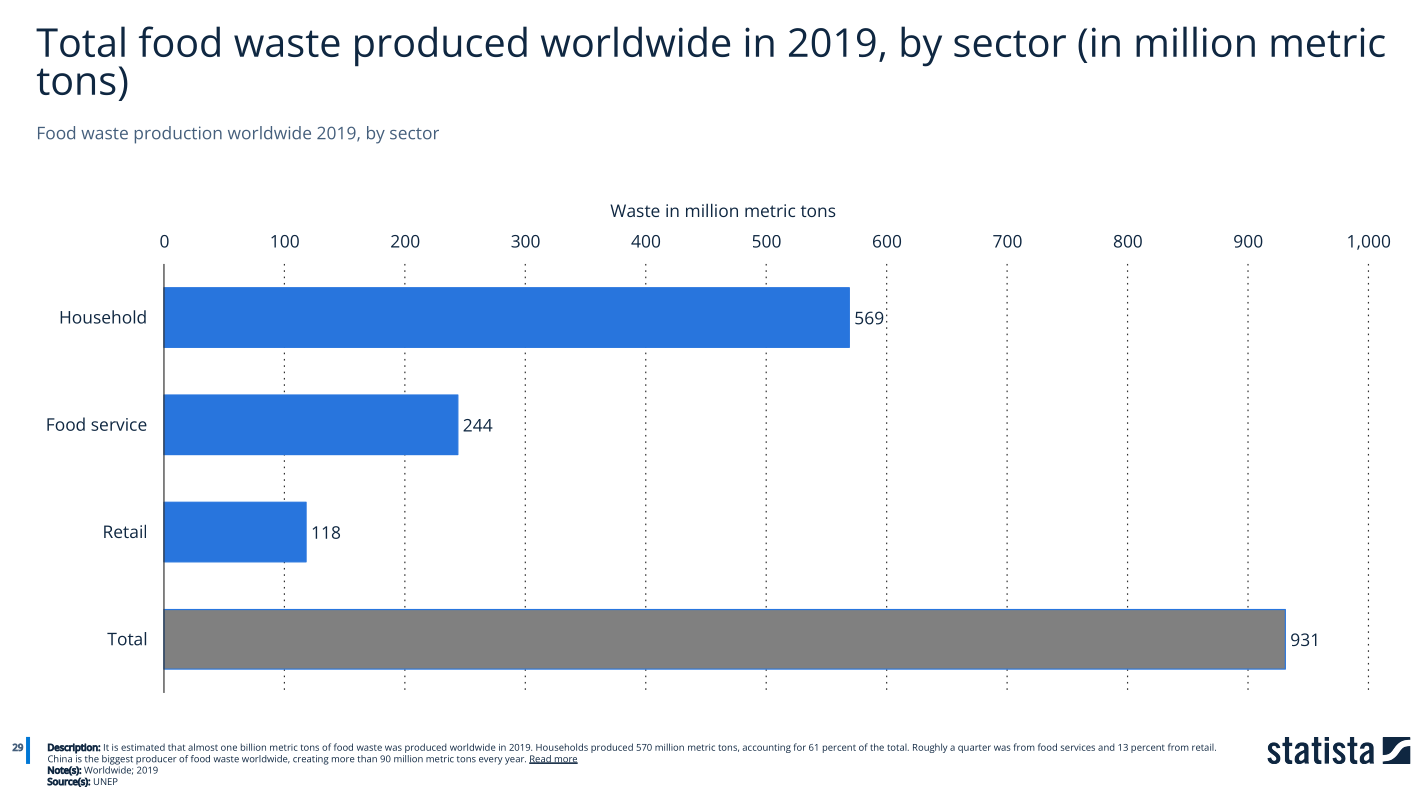
\includegraphics[width=.9\linewidth]{../plots/statistics/statistic_food_waste_by_sector_2019.png}
\caption{\label{fig:orgd4b1d00}Παγκόσμια παραγωγή υπολειμμάτων τροφών ανά τομέα}
\end{figure}

Η Ελλάδα είναι η χώρα με την δεύτερη μεγαλύτερη παραγωγή οικιακών \acrshort{fw} κατά κεφαλήν παγκοσμίως (142 κιλά/άτομο ετησίως) (\citeprocitem{37}{“Statista - The Statistics Portal” n.d.}) . Η παραγωγή \acrshort{fw}, ειδικά στον τομέα της κατανάλωσης, όπου βρίσκονται τα οικιακά υπολείμματα, καθώς και αυτά της εστίασης, είναι πολύ συχνά αναπόφευχτη. Οπότε, παρόλο που με πιο σωστές πρακτικές θα μπορούσαν να παράγονται λιγότερα υπολείμματα, η ανάπτυξη τεχνολογιών αξιοποίησης των \acrshort{fw} είναι πάρα πολύ σημαντικές. Οι τεχνολογίες αυτές θα πρέπει να είναι εύκολα εφαρμόσιμες και οικονομικές και η κλιμάκωση τους να είναι εφικτή.

Η αγορά της διαχείρισης αποβλήτων είναι αρκετά μεγάλη (υπολογίζεται περίπου στα 1293 δις δολλάρια ετησίως από μία μελέτη του 2022), ενώ προβλέψεις λένε πως θα φτάσει τα 2000 δις μέχρι το 2030. Κομμάτι της ανάπτυξης αυτής, θα πρέπει να είναι και η ανάπτυξη βιώσιμων τεχνολογιών αξιοποίησης απορριμμάτων, καθώς αυτή την στιγμή, με εξαίρεση τα απορρίμματα τα οποία είναι ανακυκλώσιμα, οι βασικές τεχνολογίες που εφαρμόζονται είναι η ανάκτηση ενέργειας μέσω καύσης και η διάθεση των απορριμμάτων σε \acrfull{xyta} όπως φαίνεται και στο \figurename  \ref{fig:org15aaa3d} (\citeprocitem{37}{“Statista - The Statistics Portal” n.d.}).

\begin{figure}[htbp]
\centering
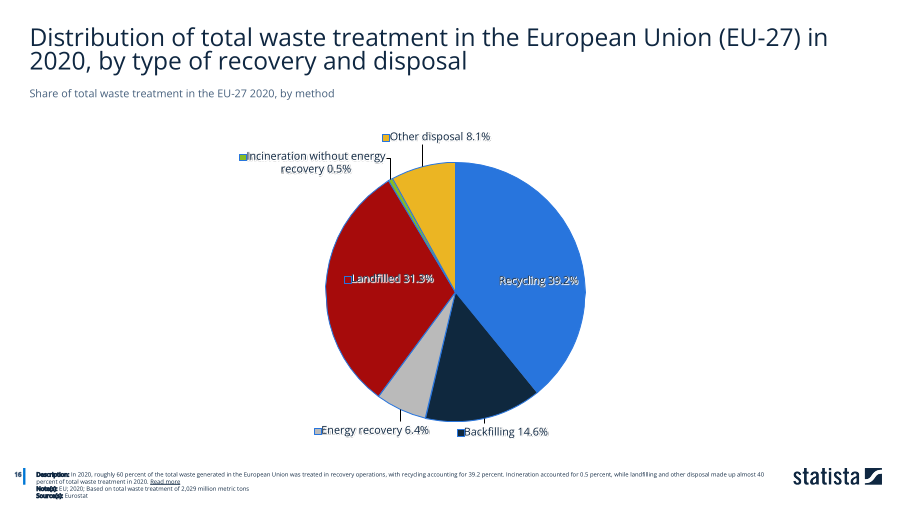
\includegraphics[width=.9\linewidth]{../plots/statistics/statistic_waste_treatment_technologies_europe_2020.png}
\caption{\label{fig:org15aaa3d}Τεχνολογίες επεξεργασίας απορριμμάτων στην Ευρωπαική Ένωση}
\end{figure}

Οι τεχνολογίες αυτές χρησιμοποιούνται επειδή είναι πολύ απλές και έχουν χαμηλό κόστος. Στα πλαίσια όμως της βιώσιμης ανάπτυξης και της κυκλικής οικονομίας, πρέπει τα απορρίμματα να εξετάζονται ως μία νέα πρώτη ύλη, από την οποία μπορούν να διυλιστούν προϊόντα αυξημένης αξίας.

Αυτές οι τεχνολογίες μπορεί να είναι θερμικές, όπως η πυρόλυση (\citeprocitem{28}{Pardo et al. 2023}; \citeprocitem{44}{Usmani et al. 2021}) η οποία παράγει ένα προιόν γνωστό ως biochar, το οποίο έχει πολύ χρήσιμες ιδιότητες (\citeprocitem{49}{Xu et al. 2024}; \citeprocitem{13}{Infurna, Caruso, and Dintcheva 2023}), ή η αεριοποίηση (\citeprocitem{44}{Usmani et al. 2021}; \citeprocitem{26}{Murugesan et al. 2022}), η οποία παράγει ένα μίγμα υδρογόνου και μονοξειδίου του άνθρακα γνωστό ως \acrfull{syngas}, το οποίο μπορεί να χρησιμοποιηθεί ως πρώτη ύλη για πολλά προιόντα. Στο \figurename  \ref{fig:org491c91b} φαίνονται κάποια κλασσικά παραδείγματα αυτού (\citeprocitem{43}{Udaeta et al. 2007})

\begin{figure}[htbp]
\centering
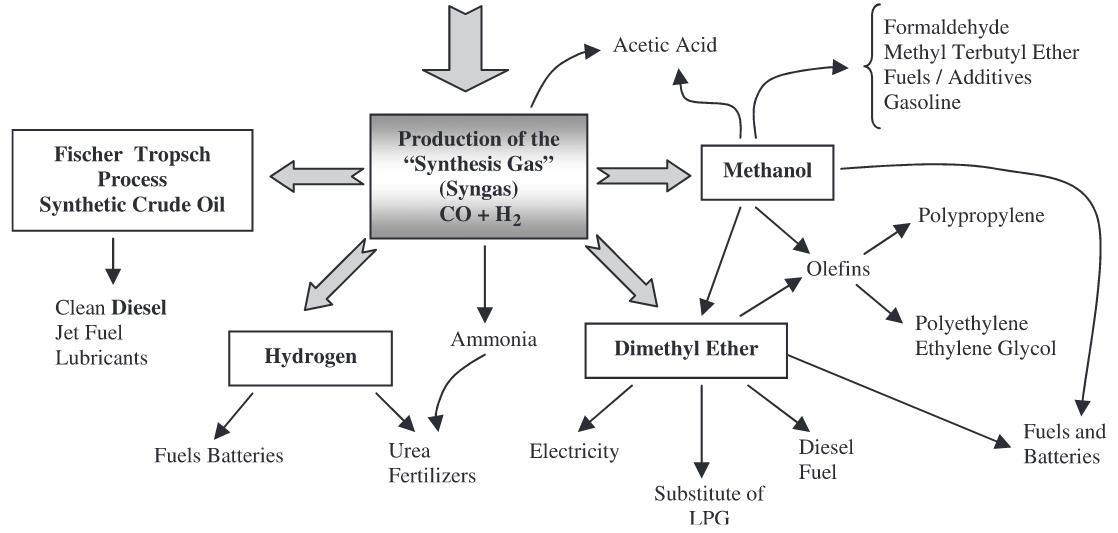
\includegraphics[width=.9\linewidth]{./gasification_products.jpg}
\caption[Προιόντα του αερίου σύνθεσης]{\label{fig:org491c91b}Προιόντα του αερίου σύνθεσης (\citeprocitem{43}{Udaeta et al. 2007})}
\end{figure}

Εκτός από θερμικές τεχνολογίες, υπάρχει μεγάλο ενδιαφέρον στις βιολογικές τεχνολογίες. Αυτές μπορεί να είναι αερόβιες, όπως η κομποστοποίηση, η οποία παράγει ένα εδαφοβελτιωτικό προιόν (\citeprocitem{6}{Cerda et al. 2018}), ή αναερόβιες όπως η αναερόβια χώνευση, η οποία έχει ως κύριο προιόν το βιοαέριο, ένα μίγμα μεθανίου και διοξειδίου του άνθρακα που μπορεί να χρησιμοποιηθεί ως βιοκαύσιμο (\citeprocitem{21}{Ma et al. 2018}; \citeprocitem{48}{Xu et al. 2018}), ή διάφορες διεργασίες ζύμωσης. Σε αυτές υπάγονται η αλκοολική ζύμωση, μία από τις πιό ευρέως χρησιμοποιούμενες τεχνολογίες αξιοποίησης απορριμμάτων (\citeprocitem{1}{Anwar Saeed et al. 2018}; \citeprocitem{33}{Roukas and Kotzekidou 2022}), η σκοτεινή ζύμωση για την παραγωγή υδρογόνου (\citeprocitem{51}{Yasin et al. 2013}; \citeprocitem{23}{Mohanakrishna et al. 2023}), ή οι ζυμώσεις με σκοπό την παραγωγή μονομερών για βιοπολυμερή όπως το \acrfull{pla} (\citeprocitem{31}{Rajesh Banu and Godvin Sharmila 2023}; \citeprocitem{29}{Pleissner et al. 2017}) .

Η παρούσα μελέτη θα εστιάσει στην \acrfull{ad}, καθώς είναι μία τεχνολογία με μεγάλο δείκτη ετοιμότητας \acrfull{trl} (\citeprocitem{22}{Mankins, n.d.}), η οποία έχει εφαρμοστεί επιτυχώς σε μεγάλη κλίμακα και είναι οικονομική.

Η \acrshort{ad} είναι μία αναερόβια βιολογική διεργασία η οποία διακρίνεται σε 4 στάδια. Στο πρώτο στάδιο, το αρχικό υπόστρωμα της διεργασίας, το οποίο συχνά αποτελείται από περίπλοκα πολυμερή όπως οι υδατάνθρακες, οι πρωτείνες και τα λιπίδια, υδρολύονται σε απλούστερες ενώσεις. Αυτές μπορούν να χρησιμοποιηθούν από τα οξεογόνα βακτήρια τα οποία τα μετατρέπουν σε \acrfull{vfa} όπως το οξικό οξύ, το προπιονικό οξύ, το βουτηρικό οξύ ή το γαλακτικό οξύ και σε αλκοόλες όπως η αιθανόλη. Στο 3ο στάδιο, οι ενώσεις αυτές μετατρέπονται σε οξικό οξύ, υδρογόνο και διοξείδιο του άνθρακα κατά την διεργασία της οξικογένεσης, ενώ τελικά, το οξικό οξύ μετατρέπεται σε μεθάνιο από μία κατηγορία μεθανογόνων μικροοργανισμών ενώ το υδρογόνο και το διοξείδιο του άνθρακα μετατρέπονται σε μεθάνιο από μία άλλη κατηγορία μεθανογόνων. Τα στάδια αυτά φαίνονται και στο \figurename \ref{fig:orgb4b5e30} (\citeprocitem{11}{Grippi, Clemente, and Bernal 2020}) .

\begin{figure}[htbp]
\centering
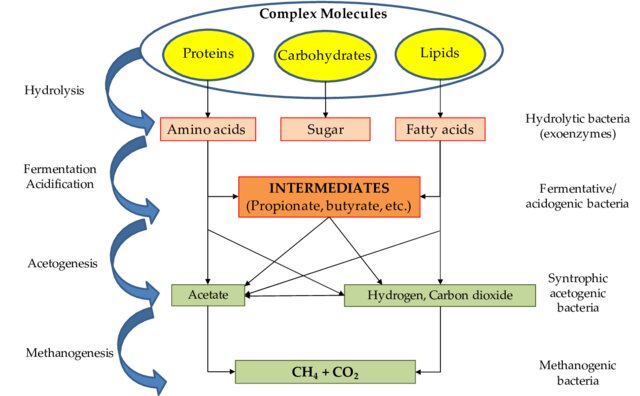
\includegraphics[width=.9\linewidth]{./anaerobic_digestion_phases.jpg}
\caption[Φάσεις της αναερόβιας χώνευσης]{\label{fig:orgb4b5e30}Φάσεις της αναερόβιας χώνευσης (\citeprocitem{11}{Grippi, Clemente, and Bernal 2020})}
\end{figure}

Ακόμη, είναι μία πολύ καλή τεχνολογία για την αξιοποίηση των \acrshort{fw} καθώς είναι πλούσια σε οργανική ύλη, η οποία είναι εύκολα αποδομήσιμη αλλά και σε θρεπτικά στοιχεία όπως το άζωτο, με υψηλότερο C/N από πολλά υποστρώματα. Λόγω αυτών, μπορούν να μετατραπούν πολύ αποτελεσματικά σε βιοαέριο (\citeprocitem{21}{Ma et al. 2018}).

Επιπροσθέτως, η \acrshort{ad} λύνει και άλλο ένα από τα σημαντικά προβλήματα του 21ου αιώνα, το οποίο είναι η ενέργεια. Αυτή τη στιγμή, πάνω από το \(80 \%\) της ενέργειας που καταναλώνεται παγκοσμίως βασίζεται σε μη ανανεώσιμες πηγές όπως το πετρέλαιο και το φυσικό αέριο. Οι ενεργειακές απαιτήσεις παγκοσμίως έχουν μία συνεχή αύξηση, ενώ οι πρώτες ύλες αυτές εξαλείφονται (\citeprocitem{37}{“Statista - The Statistics Portal” n.d.}) . Οπότε, τεχνολογίες παραγωγής ενέργειας από ανανεώσιμες πηγές, οι οποίες να έχουν το δυναμικό να αντικαταστήσουν τις πηγές αυτές θα γίνουν απαραίτητες τα επόμενα χρόνια. Οι περισσότερες τεχνολογίες ανανεώσιμης ενέργειας (πχ αιολική, ηλιακή ή υδροηλεκτρική ενέργεια) έχουν δυσκολία να φτάσουν τέτοια επίπεδα και για αυτό χρησιμοποιούνται επικουρικά σε μία κύρια πηγή ενέργειας (αυτή τη στιγμή, περίπου το \(30 \%\) της παγκόσμιας παραγωγής ηλεκτρισμού οφείλεται σε τέτοιες πηγές) (\citeprocitem{37}{“Statista - The Statistics Portal” n.d.}) . Τα υπολείμματα τροφών από την άλλη είναι άφθονα οπότε θεωρείται πως με μία αποτελεσματική επεξεργασία θα μπορέσουν να καλύψουν ένα πολύ σημαντικό ποσοστό της παγκόσμιας ανάγκης σε ενέργεια.

Στο \figurename \ref{fig:org66b7304} φαίνεται η παγκόσμια παραγωγή ενέργειας από βιοαέριο τα τελευταία 15 χρόνια, η οποία έχει ραγδαία αύξηση (\citeprocitem{37}{“Statista - The Statistics Portal” n.d.}) .

\begin{figure}[htbp]
\centering
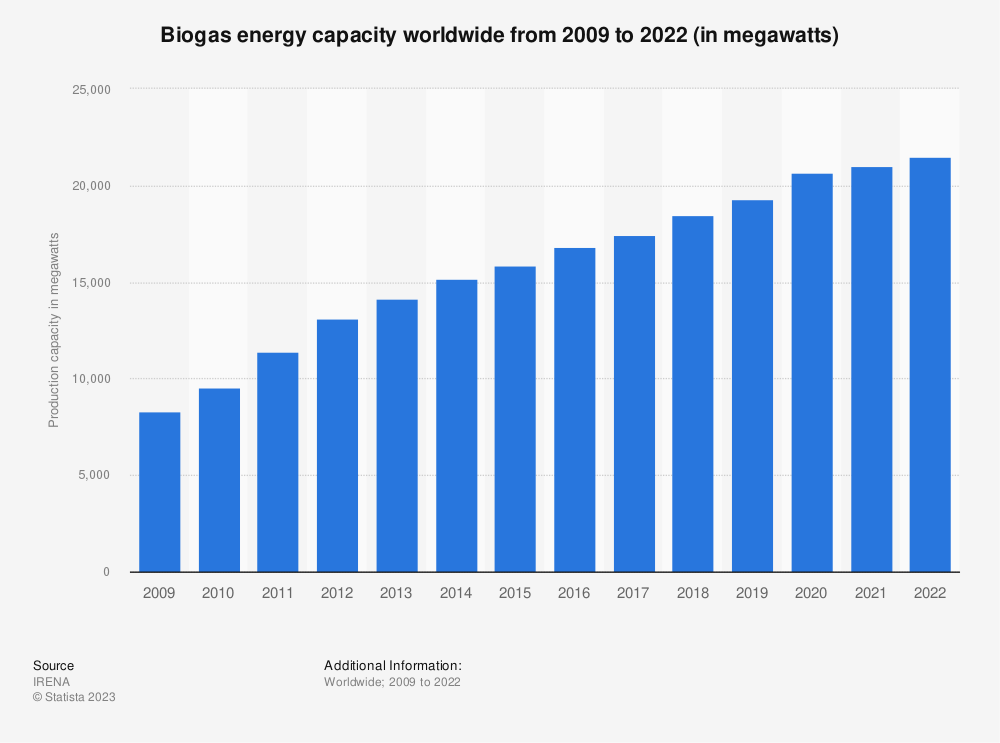
\includegraphics[width=.9\linewidth]{../plots/statistics/statistic_id1032922_global-biogas-energy-capacity-2009-2022.png}
\caption{\label{fig:org66b7304}Παγκόσμια παραγωγή ενέργειας από βιοαέριο}
\end{figure}

Βέβαια, η \acrshort{ad} έχει και κάποια σημαντικά προβλήματα. Ο βασικός περιορισμός της είναι η ευαισθησία των μεθανογόνων μικροοργανισμών στις περιβαλλοντικές συνθήκες. Λόγω της ευαισθησίας τους, η \acrshort{ad} λειτουργεί στις βέλτιστες συνθήκες αυτών. Αυτό όμως οδηγεί στην λιγότερο αποτελεσματική διεξαγωγή των άλλων σταδίων. Το κυριότερο πρόβλημα που δημιουργείται είναι πως η υδρόλυση μπορεί μεν να διεξαχθεί, αλλά γίνεται σε πολύ αργό ρυθμό, καθιστώντας την το περιοριστικό στάδιο της \acrshort{ad} και τον λόγο για τον οποίο θεωρείται μία αρκετά αργή διεργασία. Ένα αντίστοιχο πρόβλημα υπάρχει και στο στάδιο της οξεογένεσης, όπου οι μικροοργανισμοί δεν λειτουργούν στις βέλτιστες συνθήκες τους και μπορούν να ακολουθήσουν μόνο ένα μεταβολικό μονοπάτι, το οποίο ενεργοποιείται στις συνθήκες που λειτουργούν. Έτσι, η οξεογένεση είναι πιθανόν να μην είναι ιδιαίτερα αποδοτική. Παρόλα αυτά, σε ορισμένες περιπτώσεις, ο ρυθμός της οξεογένεσης ξεπερνάει αυτόν της μεθανογένεσης (ο οποίος είναι γενικά αργός), με αποτέλεσμα να παράγονται υπερβολικές ποσότητες από \acrshort{vfa}, το οποίο οδηγεί σε οξίνιση του αντιδραστήρα και κατάρρευση της διεργασίας καθώς οι μεθανογόνοι δεν μπορούν να λειτουργήσουν σε εκείνες τις τιμές pH (\citeprocitem{44}{Usmani et al. 2021}; \citeprocitem{3}{Azbar, Ursillo, and Speece 2001}; \citeprocitem{56}{Zoetemeyer et al. 1982}).

Ένας τρόπος να επιλυθεί το πρόβλημα αυτό είναι ο διαχωρισμός των σταδίων της υδρόλυσης και της ζύμωσης, σε μία διεργασία δύο (\citeprocitem{30}{Pohland and Ghosh 1971}) ή τριών (\citeprocitem{54}{Zhang et al. 2017}) σταδίων. Αυτό που πετυχαίνεται με τον διαχωρισμό αυτόν είναι να λειτουργούν όλα τα στάδια της διεργασίας στο βέλτιστο σημείο λειτουργίας τους και άρα να είναι πολύ πιο αποτελεσματικά. Επιπροσθέτως, ο αντιδραστήρας δεν οξινίζεται κατά την διάρκεια της μεθανογένεσης, με αποτέλεσμα η διεργασία να είναι πολύ πιο σταθερή. Όμως, υπάρχει το πρόβλημα πως οι διεργασίες αυτές έχουν υψηλότερο κόστος, λόγω του περισσότερου εξοπλισμού, αλλά και πολυπλοκότητας της διεργασίας. Για τον λόγο αυτόν, η διεργασία αναερόβιας χώνευσης πολλαπλών σταδίων έχει πολύ χαμηλότερο \acrshort{trl} και δεν έχει εφαρμοστεί ευρέως σε μεγάλη κλίμακα (\citeprocitem{3}{Azbar, Ursillo, and Speece 2001}; \citeprocitem{45}{Wu et al. 2022}; \citeprocitem{21}{Ma et al. 2018}; \citeprocitem{44}{Usmani et al. 2021}) .

Η υδρόλυση αποτελεί σημαντικό στάδιο της επεξεργασίας \acrshort{fw}, καθώς έχουν υψηλή περιεκτικότητα σε βιοπολυμερή. Αυτή μπορεί να γίνει θερμικά, μηχανικά, χημικά ή ενζυμικά (\citeprocitem{36}{Srisowmeya, Chakravarthy, and Nandhini Devi 2020}; \citeprocitem{15}{Kavitha et al. 2017}; \citeprocitem{21}{Ma et al. 2018}). Συνήθως η υδρόλυση γίνεται ενζυμικά καθώς έχει καταγραφεί πως επιφέρει τις υψηλότερες αποδόσεις και δεν παράγει προϊόντα τοξικά για τους μικροοργανισμούς. Ακόμη, είναι η μόνη που μπορεί να γίνει παράλληλα με την οξεογένεση για την περίπτωση της αναερόβιας χώνευσης σε 2 στάδια (\citeprocitem{52}{Zhang et al. 2020}; \citeprocitem{12}{Han et al. 2016}; \citeprocitem{21}{Ma et al. 2018}) . Παρόλα αυτά, το υψηλό κόστος των ενζυμικών σκευασμάτων καθιστά αυτή την τεχνολογία απαγορευτική σε μεγάλη κλίμακα. Για αυτό, υπάρχει αρκετή έρευνα γύρω από τεχνολογίες μείωσης του κόστους της ενζυμικής υδρόλυσης για την πιο αποτελεσματική λειτουργία της διεργασίας αυτής (\citeprocitem{57}{Zou et al. 2020}; \citeprocitem{41}{Uçkun Kiran, Trzcinski, and Liu 2015}; \citeprocitem{34}{dos Santos Ferreira et al. 2020}; \citeprocitem{29}{Pleissner et al. 2017}). Μια υποσχόμενη και οικονομική λύση είναι η χρήση σκευασμάτων τα οποία περιέχουν ένζυμα αλλά και μικροοργανισμούς. Αυτά τα σκευάσματα επιτρέπουν την αποτελεσματική υδρόλυση των \acrshort{fw} αλλά ταυτόχρονα και μία ζύμωση για παραγωγή χρήσιμων προϊόντων, όπως η αιθανόλη και τα \acrshort{vfa}. Αυτά μπορούν να ανακτηθούν ως έχουν, ή να χρησιμοποιηθούν σε διάφορες βιοδιεργασίες, όπως η \acrshort{ad}. Ένα τέτοιο υπόστρωμα μπορεί να βελτιώσει την σταθερότητα μίας αναερόβιας χώνευσης αφού περιορίζονται τα στάδια της υδρόλυσης και οξεογένεσης και ευνοείται η δράση των μεθανογόνων μικροοργανισμών (\citeprocitem{44}{Usmani et al. 2021}).

Ο σκοπός της παρούσας μελέτης είναι αρχικά να κάνει μία βιβλιογραφική ανασκόπηση των τεχνολογιών \acrshort{ad} σε πολλαπλά στάδια. Με βάση αυτήν θα αναπτυχθεί μία διεργασία αξιοποίησης υπολειμμάτων τροφών, αξιοποιώντας ένα \acrfull{mix}, η οποία να είναι οικονομικά βιώσιμη αλλά ταυτόχρονα αποτελεσματική. Αρχικά, θα αξιολογηθεί η ποιότητα της υδρόλυσης καθώς και της οξεογένεσης κατά την διεργασία αυτή σε εργαστηριακή κλίμακα, όπου υπάρχει καλός έλεγχος παραμέτρων όπως η θερμοκρασία και η ποσότητα του \acrshort{mix}. Έπειτα, θα εξεταστεί η κλιμάκωση της διεργασίας σε πιλοτική κλίμακα εξετάζοντας την ποσότητα του \acrshort{mix} και την παροχή νερού ως λειτουργικές παραμέτρους. Τέλος, θα διερευνηθεί η δυνατότητα αξιοποίησης της παραγόμενης υγρής εκροής για την παραγωγή μεθανίου σε αναερόβιους αντιδραστήρες εργαστηριακής κλίμακας.

Η δομή της εργασίας θα είναι ως εξής: Στην συνέχεια του πρώτου μέρους θα γίνει η βιβλιογραφική ανασκόπηση, η οποία θα χωριστεί σε 4 κεφάλαια. Αρχικά, στο \autoref{sec:anaerobic_digestion} θα γίνει μία πιο αναλυτική παρουσίαση της \acrshort{ad} και των προβλημάτων που δημιουργούνται αν όλα τα στάδια αυτής γίνονται ταυτόχρονα. Σκοπός αυτού είναι η ανάδειξη της σημασίας της \acrshort{ad} σε πολλαπλά στάδια. Έτσι, τα επόμενα κεφάλαια θα εστιάσουν στα στάδια της \acrshort{ad} αν αυτά διεξαχθούν ξεχωριστά. Στο \autoref{sec:fw_pretreatment} θα αναλυθούν όλες οι μεθόδοι προεπεξεργασίας υπολειμμάτων τροφών που έχουν βρεθεί στην βιβλιογραφία για να υδρολύσουν πιο αποτελεσματικά τα \acrshort{fw}, με τα πλεονεκτήματα και τα μειονεκτήματα τους, ενώ στο \autoref{sec:enzymes} θα δωθεί ιδιαίτερη έμφαση στην ενζυμική υδρόλυση, και στις προσπάθειες μείωσης του κόστους αυτής. Το \autoref{sec:acidogenesis} θα εστιάσει στην οξεογένεση και θα αναφέρει όλα τα διαθέσιμα μεταβολικά μονοπάτια αυτής και πως καθορίζεται ποιο θα επικρατήσει με βάση τις λειτουργικές συνθήκες. Ακόμη, θα αναφερθεί η χρησιμότητα του κάθε μεταβολικού προιόντος για την \acrshort{ad} για να αποφανθεί το βέλτιστο μονοπάτι. Τέλος, στο \autoref{sec:methanogenesis} θα μελετηθούν η οξικογένεση και η μεθανογένεση. Τα 2 αυτά στάδια δεν θα διαχωριστούν, καθώς στην πράξη, το ένα εξαρτάται από το άλλο και γίνονται συνεργιστικά.

Έχοντας τις πληροφορίες αυτές, μπορεί στο δεύτερο μέρος, να γίνει μία ανάλυση των πειραματικών αποτελεσμάτων της εργασίας και να προκύψουν κάποια συμπεράσματα από αυτά. Συγκεκριμένα, στο \autoref{sec:materials_methods} θα αναλυθούν οι πειραματικές διαδικασίες που χρησιμοποιήθηκαν καθώς και οι πρώτες ύλες που χρειάστηκαν. Στο \autoref{sec:result_analysis} θα αναφερθεί τι αποτελέσματα είχε ο κάθε πειραματικός κύκλος και πως αυτά αναλύθηκαν με σκοπό στο \autoref{sec:result_discussion} να γίνει η παράθεση των τελικών αποτελεσμάτων κάθε κύκλου και μία συζήτηση αυτών. Έτσι θα προκύψουν κάποια συμπεράσματα καθώς και προτάσεις για περαιτέρω έρευνα στο αντικείμενο αυτό, τα οποία θα παρατεθούν στο \autoref{sec:conclusion}.

\chapter{Αναερόβια Χώνευση}
\label{sec:org371f5f3}
\label{sec:anaerobic_digestion}

Η αναερόβια χώνευση είναι μία αναερόβια βιολογική διεργασία η οποία μετατρέπει περίπλοκη οργανική ύλη σε μεθάνιο και διοξείδιο του άνθρακα με βάση τον μηχανισμό του σχήματος \ref{fig:orgb4b5e30}. Η διεργασία αυτή έχει πολλά πλεονεκτήματα, όπως η απλότητα της λειτουργίας, το χαμηλό σχετικά λειτουργικό κόστος (χρειάζεται μόνο η διατήρηση της θερμοκρασίας σε ένα σταθερό επίπεδο) και την παραγωγή ενός πολύ αποτελεσματικού ενεργειακού φορέα, του μεθανίου (\citeprocitem{36}{Srisowmeya, Chakravarthy, and Nandhini Devi 2020}). Για αυτούς τους λόγους μάλιστα έχει δει ραγδαία ανάπτυξη τα τελευταία χρόνια (\citeprocitem{37}{“Statista - The Statistics Portal” n.d.}) .

Όμως, παραμένει περιορισμένη σε μεγάλο βαθμό από τα λειτουργικά της προβλήματα (\citeprocitem{36}{Srisowmeya, Chakravarthy, and Nandhini Devi 2020}). Αρχικά, είναι μία αργή διεργασία. Αυτό οφείλεται εν μέρει στους μεθανογόνους μικροοργανισμούς, οι οποίοι θέλουν ο \acrfull{hrt} να είναι μεγάλος για να μπορέσουν να αναπτυχθούν και να μην εκπλυθούν. Αλλά, για τα περισσότερα υποστρώματα, το περιοριστικό στάδιο της διεργασίας είναι η υδρόλυση και διαλυτοποίηση, δηλαδή η διάσπαση των στερεών και μακρομερών σωματιδίων σε διαλυτές ενώσεις, οι οποίες μπορούν να μεταβολιστούν. Στην περίπτωση των υπολειμμάτων τροφών, ένα μεγάλο ποσό της οργανικής ύλης βρίσκεται σε σωματιδιακή μορφή και δεν είναι διαλυτό. Είναι στην πλειοψηφία του ένα εύκολα υδρολύσιμο υπόστρωμα, αλλά αν η υδρόλυση γίνει κατά την διάρκεια της χώνευσης, επιβραδύνει τον χρόνο που διαρκεί η χώνευση (\citeprocitem{15}{Kavitha et al. 2017}; \citeprocitem{21}{Ma et al. 2018}; \citeprocitem{44}{Usmani et al. 2021}) . Αυτό γίνεται επειδή κατά την λειτουργία ενός χωνευτήρα, οι λειτουργικές συνθήκες ρυθμίζονται στις βέλτιστες των μεθανογόνων μικροοργανισμών, οι οποίοι είναι οι πιο ευαίσθητοι. Αυτές είναι συνήθως στη μεσόφιλη περιοχή της θερμοκρασίας (35-37 \(^oC\)) και σε pH κοντά στο ουδέτερο (6.4-8.0). Αντιθέτως, η βέλτιστη λειτουργία της υδρόλυσης από τους ήδη υπάρχοντες μικροοργανισμούς στην λάσπη είναι βέλτιστη σε πολύ πιο όξινα pH (\citeprocitem{55}{Zhang et al. 2019}; \citeprocitem{54}{Zhang et al. 2017}) και τα σύνηθη υδρολυτικά ένζυμα που εκκρίνονται από τους μικροοργανισμούς αυτούς λειτουργούν βέλτιστα σε υψηλότερες θερμοκρασίες (\citeprocitem{21}{Ma et al. 2018}; \citeprocitem{52}{Zhang et al. 2020}; \citeprocitem{5}{Cekmecelioglu and Uncu 2013}) . Για τους λόγους αυτούς, είναι συχνό να γίνεται κάποια προεπεξεργασία πριν την αναερόβια χώνευση, η οποία αποσκοπεί στην υδρόλυση και διαλυτοποίηση του υποστρώματος (\citeprocitem{7}{Cesaro and Belgiorno 2014}; \citeprocitem{10}{Graunke and Wilkie 2014}; \citeprocitem{36}{Srisowmeya, Chakravarthy, and Nandhini Devi 2020}; \citeprocitem{21}{Ma et al. 2018}) .

Το άλλο βασικό πρόβλημα της αναερόβιας χώνευσης, είναι η ανισορροπία στους ρυθμούς της αντίδρασης. Στην περίπτωση που και τα 4 στάδια γίνονται ταυτόχρονα, μία ευσταθής συνθήκη λειτουργίας, θα ήταν όλα τα στάδια να έχουν τον ίδιο ρυθμό, ώστε ότι παράγεται να καταναλώνεται. Στην πράξη όμως, αυτό δεν συμβαίνει. Οι οξεογόνοι μικροοργανισμοί συχνά μεταβολίζουν το υπόστρωμα τους πιο γρήγορα από τους μεθανογόνους, οπότε σε πολλές περιπτώσεις μπορεί να παρατηρηθεί συσσώρευση πτητικών λιπαρών οξέων. Η συσσώρευση αυτή σημαίνει πως θα μειωθεί το pH του αντιδραστήρα σε ένα επίπεδο που θα ανασχεθεί η λειτουργία των μεθανογόνων μικροοργανισμών και σταδιακά θα σταματήσει η παραγωγή μεθανίου, κάτι που θα συντελέσει στην κατάρρευση του συστήματος. Η ανισορροπία αυτή στους ρυθμούς μπορεί όμως να συντελέσει και άλλο ένα πρόβλημα. Εκτός από \acrshort{vfa}, παράγεται και υδρογόνο κατά την οξεογένεση. Η υψηλή μερική πίεση υδρογόνου στο σύστημα είναι επίσης ανασχετική για τους μεθανογόνους και μπορεί να οδηγήσει το σύστημα σε κατάρρευση. Λόγω των προβλημάτων αυτών, το σύστημα αναερόβιας χώνευσης ενός σταδίου, δεν έχει ιδιαίτερα μεγάλη σταθερότητα (\citeprocitem{36}{Srisowmeya, Chakravarthy, and Nandhini Devi 2020}; \citeprocitem{48}{Xu et al. 2018}; \citeprocitem{3}{Azbar, Ursillo, and Speece 2001}; \citeprocitem{54}{Zhang et al. 2017}) .

Ο συμβατικός τρόπος που επιλύεται αυτό είναι o χαμηλός \acrfull{olr}. Αν το σύστημα τροφοδοτείται με μικρή ποσότητα υποστρώματος, θα είναι χαμηλός γενικά ο ρυθμός της οξεογένεσης, με αποτέλεσμα να είναι πιο δύσκολο να δημιουργηθεί αστάθεια. Βέβαια, η χρήση πολύ χαμηλού \acrshort{olr} είναι προβληματική επειδή περιορίζει σημαντικά τον ρυθμό επεξεργασίας του αποβλήτου. Ειδικά στην περίπτωση των υπολειμμάτων τροφών τα οποία παράγονται σε πολύ μεγάλους ρυθμούς, θα ήταν ιδανικό ο χωνευτήρας να λειτουργεί σε υψηλό ρυθμό οργανικής φόρτισης. Ένας τρόπος να αυξηθεί ο \acrlong{olr} είναι η χρήση ενός ταχύρυθμου αντιδραστήρα όπως ο \acrfull{uasb}. Στον αντιδραστήρα αυτόν, η λάσπη που δημιουργείται είναι κοκκώδης λόγω του σχηματισμού βιοφίλμ. Αυτό έχει ως αποτέλεσμα οι μεθανογόνοι μικροοργανισμοί να προστατεύονται καλύτερα από τις εξωτερικές συνθήκες και η διεργασία να έχει μεγαλύτερη σταθερότητα. Αυτό επιτρέπει την αύξηση του \acrshort{olr} (\citeprocitem{3}{Azbar, Ursillo, and Speece 2001}; \citeprocitem{45}{Wu et al. 2022}; \citeprocitem{46}{Wu et al. 2016}) .

Όμως, ο πιο αποτελεσματικός τρόπος να αυξηθεί ο \acrlong{olr} σε έναν αντιδραστήρα αναερόβιας χώνευσης είναι μία διάταξη σε δύο στάδια (\citeprocitem{30}{Pohland and Ghosh 1971}; \citeprocitem{56}{Zoetemeyer et al. 1982}; \citeprocitem{3}{Azbar, Ursillo, and Speece 2001}). Σε αυτή, διαχωρίζονται τα στάδια της υδρόλυσης και οξεογένεσης από την μεθανογένεση. Ως αποτέλεσμα, η εκροή του οξεογενή αντιδραστήρα μπορεί να υποστεί μία ρύθμιση pH στην περιοχή που λειτουργούν βέλτιστα οι μεθανογόνοι και εφόσον έχει ολοκληρωθεί ήδη η οξεογένεση, δεν υπάρχει ο κίνδυνος να οξινιστεί ο αντιδραστήρας, κάτι που θα οδηγούσε στην κατάρρευση του. Έτσι, τα συστήματα αυτά είναι πολύ πιο σταθερά και μπορούν να λειτουργήσουν σε μεγαλύτερα \acrshort{olr} πολύ αποτελεσματικά (\citeprocitem{30}{Pohland and Ghosh 1971}; \citeprocitem{45}{Wu et al. 2022}). Ακόμη ένα πλεονέκτημα της διάταξης αυτής είναι πως διαχωρίζοντας τα στάδια της υδρόλυσης και της οξεογένεσης, το οποίο επιτρέπει την λειτουργία τους σε πιο επιθυμητές συνθήκες. Η οξεογένεση είναι μία περίπλοκη διεργασία η οποία μπορεί να ακολουθήσει πολλά μεταβολικά μονοπάτια ανάλογα με τις συνθήκες στις οποίες θα διεξαχθεί. Η επιλογή του βέλτιστου μονοπατιού εξαρτάται από πολλούς παράγοντες και θα αναλυθεί περαιτέρω στο \autoref{sec:acidogenesis}, αλλά είναι κάτι που είναι εφικτό μόνο σε συστήματα δύο φάσεων. Η βέλτιστη λειτουργία της υδρόλυσης είναι λίγο πιο καθορισμένη. Όμως, συνήθως δεν λαμβάνεται υπόψην στα συστήματα δύο φάσεων, καθώς συνήθως καθορίζονται από την οξεογένεση. Καθώς η υδρόλυση λειτουργεί βέλτιστα σε όξινα pH, η λειτουργία της στο σύστημα αυτό είναι σίγουρα πιο αποτελεσματική από την υδρόλυση στο σύστημα μίας φάσης (\citeprocitem{45}{Wu et al. 2022}; \citeprocitem{21}{Ma et al. 2018}; \citeprocitem{3}{Azbar, Ursillo, and Speece 2001}; \citeprocitem{44}{Usmani et al. 2021}). Στην βιβλιογραφία, υπάρχουν και κάποια συστήματα αναερόβιας χώνευσης τριών σταδίων (\citeprocitem{44}{Usmani et al. 2021}; \citeprocitem{55}{Zhang et al. 2019}; \citeprocitem{54}{Zhang et al. 2017}; \citeprocitem{16}{Kim and Kim 2013}), στα οποία λειτουργεί και η υδρόλυση ξεχωριστά και στο βέλτιστο σημείο λειτουργίας της. Η διεργασία αυτή είναι πιο αποτελεσματική και πιο σταθερή, αλλά ταυτόχρονη ακόμη πιο περίπλοκη. Οπότε, γενικά προτιμάται η διεργασία δύο σταδίων, ως μία ισορροπία μεταξύ πολυπλοκότητας και σταθερότητας της λειτουργίας (\citeprocitem{44}{Usmani et al. 2021}).

\chapter{Προεπεξεργασία Υπολειμμάτων Τροφών}
\label{sec:org92cf3f3}
\label{sec:fw_pretreatment}

Τα \acrshort{fw} έχουν υψηλή περιεκτικότητα σε βιοπολυμερή. Για να μπορέσουν να χρησιμοποιηθούν αποδοτικά ως ένα υπόστρωμα για διεργασίες όπως η \acrshort{ad}, απαιτείται κάποια διεργασία η οποία θα υδρολύσει το υπόστρωμα αυτό. Υπάρχουν πολλές τεχνολογίες για να βοηθήσουν την υδρόλυση του υποστρώματος αυτού όπως η μηχανική, θερμική, χημική ή ενζυμική προεπεξεργασία και η προεπεξεργασίες με υπερήχους και μικροκύματα.

\section{Μηχανική Επεξεργασία}
\label{sec:org9aa2bd4}
Η πιο απλή είναι η μηχανική επεξεργασία. Μία μηχανική επεξεργασία όπως ο τεμαχισμός είναι αρκετά αποτελεσματική. Ο σκοπός της είναι η ομογενοποίηση της στερεής μάζας και μείωση του μεγέθους κόκκων της ώστε να επιταχυνθούν τα επόμενα στάδια της προεπεξεργασίας. Είναι το πιο σύνηθες στάδιο προεπεξεργασίας και γίνεται ανεξαρτήτως των επόμενων σταδίων συνήθως (\citeprocitem{9}{Chen et al. 2022}; \citeprocitem{24}{Moon and Song 2011}; \citeprocitem{44}{Usmani et al. 2021}) . 

\section{Θερμική Επεξεργασία}
\label{sec:org831231b}
Η θερμική υδρόλυση βασίζεται στην αύξηση της θερμοκρασίας, με σκοπό την διάσπαση των πολυμερικών δεσμών. Είναι πολύ αποτελεσματική ως μία προεπεξεργασία για δύσκολα αποδομήσιμη βιομάζα. Στην περίπτωση των \acrshort{fw}, οι υψηλές θερμοκρασίες δεν είναι αναγκαίες για την αποικοδόμηση και μάλιστα συνήθως υποβαθμίζουν την ποιότητα του υποστρώματος καθώς καταστρέφουν οργανική ύλη και μπορεί να παράξουν προιόντα θερμικής αποδόμησης τα οποία είναι τοξικό για επόμενα βιολογικά στάδια. Ακόμη, είναι μία τεχνική με σχετικά υψηλές ενεργειακές απαιτήσεις (\citeprocitem{36}{Srisowmeya, Chakravarthy, and Nandhini Devi 2020}; \citeprocitem{7}{Cesaro and Belgiorno 2014}; \citeprocitem{21}{Ma et al. 2018}) .

\section{Επεξεργασία με Μικροκύματα}
\label{sec:orgadd9c24}
Αντίστοιχη λογική έχει και η χρήση μικροκυμάτων, η οποία αυξάνει την θερμοκρασία μέσω ενός ηλεκτρομαγνητικού πεδίου. Θεωρείται πιο αποτελεσματική από την θερμική τεχνολογία λόγω της μικρότερης κατανάλωσης ενέργειας. Επίσης, συνδυάζει θερμικά με μη θερμικά φαινόμενα. Όμως, όπως και στη περίπτωση της θερμικής υδρόλυσης, δεν επιφέρει ιδιαίτερα θετικά αποτελέσματα για την επεξεργασία \acrshort{fw} (\citeprocitem{7}{Cesaro and Belgiorno 2014}; \citeprocitem{21}{Ma et al. 2018}; \citeprocitem{36}{Srisowmeya, Chakravarthy, and Nandhini Devi 2020}) . 

\section{Επεξεργασία με Υπερήχους}
\label{sec:org6cd79d1}
Η χρήση υπερήχων βασίζεται στην δημιουργία ελεύθερων ριζών υδροξυλίου \(OH^{\cdot}\), οι οποίες διασπούν ταχύτατα τα στερεά, απελευθερώνοντας μεγάλα ποσά οργανικής ύλης. Πειράματα που έχουν χρησιμοποιήσει υπερήχους ως μία προεπεξεργασία για αναερόβια χώνευση έχουν δείξει πως βελτιώνει αρκετά την παραγωγή μεθανίου. Βέβαια, υδρολύουν μόνο σε περιορισμένο βαθμό το υπόστρωμα, με αποτέλεσμα να πρέπει να γίνει και κάποια υδρόλυση κατά την διάρκεια της χώνευσης (\citeprocitem{7}{Cesaro and Belgiorno 2014}; \citeprocitem{21}{Ma et al. 2018}) .

\section{Χημική Επεξεργασία}
\label{sec:org82beff5}
Σε ένα παρόμοιο μηχανισμό βασίζεται και η χημική τεχνολογία της οζόνωσης, καθώς η τροφοδοσία με όζον δημιουργεί και αυτή ελεύθερες ρίζες οι οποίες διασπούν την στερεή οργανική ύλη. Είναι όμως μία πιο έντονη επεξεργασία η οποία χρησιμοποιείται σε υποστρώματα τα οποία είναι πιο δύσκολα στην αποδόμηση. Στην περίπτωση των \acrshort{fw} μπορεί να οδηγήσουν σε μείωση του COD λόγω οξείδωσης ακόμη και των ζυμώσιμων σακχάρων και παραγωγής προιόντων πιο δύσκολα αποδομήσιμα από τα αρχικά, για αυτό δεν συνηθίζεται (\citeprocitem{36}{Srisowmeya, Chakravarthy, and Nandhini Devi 2020}; \citeprocitem{7}{Cesaro and Belgiorno 2014}) .

Βέβαια, η πιο συχνή κατηγορία χημικής επεξεργασίας είναι αυτή που βασίζεται στην προσθήκη οξέος ή βάσης. Η προσθήκη των ενώσεων αυτών βασίζεται στην επίτευξη ακραίων τιμών pH, στις οποίες καταρρέει η πολυμερική δομή. Στην τεχνολογία αυτή χρησιμοποιούνται ισχυρά οξέα ή βάσεις (πχ θειικό οξύ, υδροχλωρικό οξύ, καυστικό νάτριο ή ασβέστης). Η τεχνολογία αυτή είναι μακράν η πιο απλή και φθηνή τεχνολογία προεπεξεργασίας, ενώ είναι αρκετά αποτελεσματική και για αυτό χρησιμοποιείται αρκετά (\citeprocitem{7}{Cesaro and Belgiorno 2014}; \citeprocitem{21}{Ma et al. 2018}; \citeprocitem{52}{Zhang et al. 2020}). Ακόμη, για την αλκαλική υδρόλυση συγκεκριμένα, ισχύει πως αν τα \acrshort{fw} χρησιμοποιηθούν μετά για αναερόβια χώνευση, το σύστημα θα έχει αποκτήσει μεγαλύτερη αλκαλικότητα, με αποτέλεσμα να έχει καλύτερη σταθερότητα η διεργασία (\citeprocitem{36}{Srisowmeya, Chakravarthy, and Nandhini Devi 2020}) . Όμως, μπορεί να παραχθούν μη επιθυμητά προϊόντα κατά την όξινη ή αλκαλική αποδόμηση των \acrshort{fw}, όπως η φουρφουράλη, τα οποία είναι τοξικά προς μικροοργανισμούς και άρα να μειώσουν σημαντικά την απόδοση της διεργασίας (\citeprocitem{12}{Han et al. 2016}; \citeprocitem{52}{Zhang et al. 2020}; \citeprocitem{21}{Ma et al. 2018}) .

\section{Ενζυμική Επεξεργασία}
\label{sec:org2995139}
Τέλος, υπάρχει η ενζυμική επεξεργασία. Αυτή βασίζεται στην χρήση υδρολυτικών ενζύμων όπως οι υδατανθρακάσες, οι πρωτεάσες και οι λιπάσες για την διάσπαση των βιοπολυμερών. Η διεργασία αυτή δεν έχει κανένα τοξικό παραπροιόν, ήπιες συνθήκες (οι οποίες συνδέονται με το κόστος) και εξαιρετική απόδοση υδρόλυσης/βιοαποδόμησης (\citeprocitem{21}{Ma et al. 2018}; \citeprocitem{12}{Han et al. 2016}). Επίσης, είναι η μόνη προεπεξεργασία, της οποίας οι συνθήκες μπορούν να ρυθμιστούν έτσι ώστε να γίνει ταυτόχρονα με την οξεογένεση, το οποίο επιτρέπει την αναερόβια χώνευση σε 2 στάδια. Σε κάθε άλλη περίπτωση, η διεργασία πρέπει να γίνει σε τρία στάδια, το οποίο παρότι προσφέρει σταθερότητα και πιθανόν καλύτερες αποδόσεις, δημιουργεί και πολυπλοκότητα στην διεργασία (\citeprocitem{44}{Usmani et al. 2021}; \citeprocitem{21}{Ma et al. 2018}) . Παρόλα αυτά, το κόστος ενός εμπορικού ενζυμικού σκευάσματος είναι πολύ υψηλό, κάτι που καθιστά την συμβατική ενζυμική υδρόλυση μία τεχνολογία απαγορευτική σε μεγάλη κλίμακα. Για τον λόγο αυτόν, στην βιβλιογραφία υπάρχουν αρκετές μελέτες χρησιμοποιώντας πρωτοποριακές τεχνολογίες ενζυμικής υδρόλυσης χαμηλού κόστους για να λύσουν το πρόβλημα αυτό (\citeprocitem{8}{Chen et al. 2020}; \citeprocitem{54}{Zhang et al. 2017}; \citeprocitem{34}{dos Santos Ferreira et al. 2020}; \citeprocitem{29}{Pleissner et al. 2017}; \citeprocitem{38}{Suresh et al. 2020}) . Οι τεχνολογίες αυτές θα αναλυθούν σε περισσότερο βάθος στο \autoref{sec:enzymes}

\chapter{Βελτιστοποίηση της Διεργασίας της Ενζυμικής Υδρόλυσης}
\label{sec:org962c35d}
\label{sec:enzymes}

Στο \autoref{sec:fw_pretreatment} αναφέρθηκαν όλες οι τεχνολογίες προεπεξεργασία των \acrshort{fw} για να επιτευχθούν υψηλές αποδόσεις σε επόμενα βιολογικά στάδια όπως η \acrshort{ad}. Προέκυψε, πως η ενζυμική υδρόλυση/βιοαποδόμηση είναι η πιο αποτελεσματική καθώς δεν έχει παραπροιόντα, χρησιμοποιεί ήπιες συνθήκες, μειώνει αποτελεσματικά τα \acrfull{ts} και αυξάνει το διαλυτό \acrfull{cod} και μπορεί να γίνει παράλληλα με την οξεογένεση. Όμως, αναφέρθηκε πως το κύριο εμπόδιο της είναι το κόστος των ενζυμικών σκευασμάτων. Για αυτό, στο κεφάλαιο αυτό θα αναφερθούν όλες οι τεχνολογίες που έχουν προταθεί στην βιβλιογραφία για την μείωση του κόστους της διεργασίας αυτής. Γενικά, κατατάσσονται σε δύο κατηγορίες:

\begin{itemize}
\item Εντατικοποίηση της διεργασίας υδρόλυσης (\acrfull{pi}) και μείωση του απαιτούμενου χρόνου υδρόλυσης, ο οποίος σε συνεχή συστήματα αντιστοιχεί στην ποσότητα ενζύμων που απαιτούνται.
\item Χρήση μικροοργανισμών, οι οποίοι στις κατάλληλες συνθήκες θα εκκρίνουν υδρολυτικά ένζυμα in-situ για την υδρόλυση
\end{itemize}

\section{Εντατικοποίηση της Διεργασίας Υδρόλυσης}
\label{sec:org753d031}
Οι μελέτες οι οποίες υπάγονται σε αυτήν την κατηγορία αποτελούν τις μελέτες οι οποίες έχουν προσπαθήσει να βελτιστοποιήσουν διάφορες συνθήκες της υδρόλυσης, με σκοπό την πιο αποτελεσματική και γρήγορη ενζυμική υδρόλυση, η οποία θα έχει χαμηλότερο κόστος.

Για παράδειγμα, οι (\citeprocitem{10}{Graunke and Wilkie 2014}) προσπάθησαν να μειώσουν πολύ τον χρόνο παραμονής στην υδρόλυση και έδειξαν ότι με βέλτιστες συνθήκες, σε περίπου 4 ώρες έχει γίνει ικανοποιητική υδρόλυση. Καθώς ο χρόνος αυτός συχνά είναι στις 24 ώρες, μία τέτοια μείωση θα μπορούσε να μειώσει σημαντικά την απαίτηση σε ένζυμα και άρα να βελτιώσει το οικονομικό προφίλ της διεργασίας (\citeprocitem{25}{Moon et al. 2009}; \citeprocitem{21}{Ma et al. 2018}; \citeprocitem{53}{Zhang, Ling, and Huo 2021}) .

Οι (\citeprocitem{38}{Suresh et al. 2020}) έκαναν μία μελέτη στην οποία προσπάθησαν να βελτιστοποίησουν μία διεργασία παραγωγής βιοαιθανόλης από απόβλητα της βιομηχανίας επεξεργασίας πατάτας λαμβάνοντας υπόψην συνθήκες όπως η ποσότητα ενζύμων που θα χρησιμοποιηθεί και η πιθανότητα χρήσης άλλων διεργασιών υδρόλυσης επικουρικά, όπως η προσθήκη HCl ή χρήση υπερήχων κατά την διεργασία.

Οι (\citeprocitem{20}{Li et al. 2019}) χρησιμοποιήσαν έναν συνδυασμό υπερήχων και ενζυμικής υδρόλυσης με σκοπό οι υπέρηχοι να κάνουν την βιομάζα πιο προσβάσιμη στα ένζυμα, με σκοπό να μειωθεί σημαντικά η ποσότητα ενζύμων που πρέπει να προστεθεί. Η μελέτη τους έδειξε πως αυτός ο συνδυασμός είναι αρκετά αποτελεσματικός.

Παρόλες τις επιτυχίες που υπάρχουν στον τομέα αυτόν, ακόμη και με σημαντική μείωση της ποσότητας ενζύμων που χρειάζονται, όσο μεγαλώνει η κλίμακα, γίνεται όλο και πιο δύσκολο η τεχνική αυτή να είναι αποτελεσματική. Οπότε, θεωρείται πως οι πιο αποτελεσματικές τεχνικές υδρόλυσης είναι στην δεύτερη κατηγορία, όπου το σύστημα τροφοδοτείται με μικροοργανισμούς και οι συνθήκες ελέγχονται ώστε να παραχθούν in-situ μεγάλες ποσότητες υδρολυτικών ενζύμων.

\section{Ζύμωση Στερεής Κατάστασης}
\label{sec:orgfc46d0c}
Η ζύμωση στερεής κατάστασης (\acrfull{ssf}) είναι μία αρκετά ενδιαφέρουσα κατηγορία ζύμωσης. Η βασική της αρχή είναι πως δεν χρησιμοποιείται νερό στον αντιδραστήρα όπου θα αναπτυχθεί ο μικροοργανισμός (ή οι μικροοργανισμοί στη περίπτωση μικτής καλλιέργειας) αλλά κάποια στερεή φάση, η οποία μπορεί να χρησιμοποιηθεί ως η τροφή του μικροοργανισμού (\citeprocitem{29}{Pleissner et al. 2017}; \citeprocitem{34}{dos Santos Ferreira et al. 2020}).

Μία από τις βασικές εφαρμογές της \acrshort{ssf} είναι η ανάπτυξη μυκήτων οι οποίοι μπορούν να εκκρίνουν μεγάλη ποσότητα ενζύμων. Η τεχνολογία αυτή για την παραγωγή υδρολυτικών ενζύμων έχει αρκετό ενδιαφέρον, καθώς είναι μία διεργασία η οποία χρησιμοποιεί συχνά απόβλητα ως πρώτη ύλη. Για παράδειγμα, μπορούν τα ίδια \acrshort{fw} που θα χρησιμοποιηθούν για την \acrshort{ad} να χρησιμοποιηθούν και στην \acrshort{ssf} (\citeprocitem{42}{Uçkun Kiran et al. 2014}). Έπειτα, η βιομάζα που έχει παραχθεί στην \acrshort{ssf} μπορεί να αναμειχθεί με τα υπόλοιπα \acrshort{fw} και το μίγμα αυτό να χρησιμοποιηθεί για διεργασίες όπως η αναερόβια χώνευση (\citeprocitem{34}{dos Santos Ferreira et al. 2020}; \citeprocitem{35}{Soares et al. 2019}). Ακόμη όμως και στην περίπτωση που δεν χρησιμοποιούνται απόβλητα, χρησιμοποιείται κάποιο φθηνό υπόστρωμα, το οποίο προσωμοιώνει το φυσικό περιβάλλον ανάπτυξης του μικροοργανισμού, και όχι κάποια καθαρή ένωση όπως η γλυκόζη. Έτσι, μπορεί να παράγει μεγάλες ποσότητες υδρολυτικών ενζύμων σε πολύ χαμηλό κόστος (\citeprocitem{41}{Uçkun Kiran, Trzcinski, and Liu 2015}; \citeprocitem{57}{Zou et al. 2020}; \citeprocitem{29}{Pleissner et al. 2017}) . 

Επιπλέον, στην διεργασία \acrshort{ssf} δεν απαιτείται κάποιο downstream processing, καθώς όλη η βιομάζα του μύκητα, η οποία είνα πλούσια σε υδρολυτικά ένζυμα, προστίθεται στον αντιδραστήρα. Ο καθαρισμός των ενζύμων είναι το δυσκολότερο κομμάτι της παραγωγής τους και ο βασικός λόγος για τον οποίο είναι ακριβά. Μία τέτοια διεργασία μπορεί να παράγει ένζυμα χωρίς αυτόν τον περιορισμό, και σε ορισμένες περιπτώσεις να είναι και πιο αποτελεσματική από την χρήση ενός εμπορικού σκευάσματος. Επιπροσθέτως, μπορεί να παραχθεί ένα μίγμα ενζύμων το οποίο είναι δύσκολο να βρεθεί ως έχει εμπορικά (\citeprocitem{57}{Zou et al. 2020}; \citeprocitem{34}{dos Santos Ferreira et al. 2020}; \citeprocitem{41}{Uçkun Kiran, Trzcinski, and Liu 2015}).

Εκτός όμως από το κόστος, η τεχνολογία αυτή έχει πολλά πλεονεκτήματα. Αρχικά, καθώς μιλάμε για στερεή φάση και όχι υδατική, ο όγκος του αντιδραστήρα που απαιτείται είναι αρκετά μικρός, το οποίο μειώνει σημαντικά το κόστος της διεργασίας. Επίσης, σε μία στερεή φάση, υπάρχει μικρότερος κίνδυνος για μόλυνση σε σχέση με την υγρή. Ακόμη, το προιόν της ζύμωσης (στην περίπτωση που εξετάζεται τα ένζυμα) προκύπτει πυκνό και χωρίς ανάγκη ακριβού διαχωρισμού στον οποίο θα απομακρυνθεί το νερό, μειώνοντας σημαντικά το κόστος οποιοδήποτε downstream processing. Επιπλέον, εφόσον δεν απομακρύνεται νερό, δεν υπάρχουν υγρά απόβλητα τα οποία απαιτούν διαχείριση (\citeprocitem{2}{Arora, Rani, and Ghosh 2018}; \citeprocitem{34}{dos Santos Ferreira et al. 2020}) . Όμως, είναι μία σχετικά καινούργια τεχνολογία, η οποία δεν έχει τόσο υψηλό \acrshort{trl} και δεν έχει αξιοποιηθεί εμπορικά σε μεγάλο βαθμό. Παρόλα αυτά, θεωρείται πως έχει πολύ μεγάλο περιθώριο εφαρμογής για διεργασίες που θέλουν ενζυμική υδρόλυση, αλλά το κόστος της την κάνει ανεπιθύμητη (\citeprocitem{2}{Arora, Rani, and Ghosh 2018}) . 

Για την διεργασία αυτή, ένα από τα πιο βασικά γένη είναι τα Aspergillus, με τα A. awamori, A. oryzae, A. terreus και A. niger να είναι τα βασικότερα στελέχη που έχουν εφαρμοστεί στην διεργασία. Έχει βρεθεί πως ο A. awamori είναι ένας από τους αποτελεσματικούς μύκητες για την παραγωγή υδατανθρακασών, ο A. oryzae είναι ένας από τους πιο αποτελεσματικούς για πρωτεάσες ενώ ο Α. terreus είναι ένας από τους πιο αποτελεσματικούς για λιπάσες (\citeprocitem{35}{Soares et al. 2019}; \citeprocitem{57}{Zou et al. 2020}). Ο λόγος που χρησιμοποιούνται μικροοργανισμοί του γένους αυτού είναι επειδή μπορούν να προσαρμωστούν εύκολα σε διάφορες περιβαλλοντικές συνθήκες και έχουν μεγάλο εύρος θερμοκρασιών και pH στα οποία μπορούν να αναπτυχθούν (από ψυχρόφιλους μέχρι 10 \(^oC\) μέχρι θερμόφιλους στους 50 \(^oC\) και από οξεόφιλους σε pH εώς και 2 μέχρι αλκαλόφιλους σε pH 11). Επίσης, μπορούν να λειτουργήσουν αποτελεσματικά ακόμη και σε συνθήκες ολιγοτροφισμού. Όλα αυτά, τους κάνουν πολύ ικανούς για την διεργασία αυτή, η οποία έχει πολύ μεγάλη σημασία στα πλαίσια της προεπεξεργασίας αποβλήτων, καθώς η ενζυμική υδρόλυση είναι η πιο αποτελεσματική τεχνολογία προεπεξεργασίας, αλλά η τιμή της είναι απαγορευτική (\citeprocitem{2}{Arora, Rani, and Ghosh 2018}; \citeprocitem{35}{Soares et al. 2019}) .

\section{Παραγωγή Υδρολυτικών Ενζύμων από Βακτήρια}
\label{sec:org610763f}
Βέβαια, εκτός από \acrshort{ssf} με χρήση μηκύτων, υδρολυτικά ένζυμα μπορούν να παραχθούν και από βακτήρια. Από το \figurename \ref{fig:orgb4b5e30} φαίνεται πως κατά την αναερόβια χώνευση, μπορεί να γίνει υδρόλυση από τα υδρολυτικά βακτήρια, τα οποία εκκρίνουν ένζυμα με αυτήν την δράση (\citeprocitem{11}{Grippi, Clemente, and Bernal 2020}). Όπως προαναφέρθηκε, οι συνθήκες της χώνευσης δεν είναι σύμφωνες με τις ιδανικές για τους μικροοργανισμούς αυτούς, οπότε η χώνευση, διεξάγεται πολύ αργά, στην περίπτωση αυτή. Όμως, ως ένα χωριστό στάδιο υδρόλυσης, οι συνθήκες αυτές μπορούν να ρυθμιστούν καλύτερα (\citeprocitem{55}{Zhang et al. 2019}; \citeprocitem{54}{Zhang et al. 2017}) . Η υδρόλυση λείτουργεί βέλτιστα σε όξινα pH (πχ 4.5-5.0) και πολλά από τα υδρολυτικά βακτήρια είναι θερμόφιλα, οπότε οι υψηλές θερμοκρασίες (πχ 45-55 \(^oC\)) μπορεί να συνεισφέρουν στην πιο αποτελεσματική υδρόλυση (\citeprocitem{47}{Xiao et al. 2018}; \citeprocitem{54}{Zhang et al. 2017}; \citeprocitem{40}{Tang et al. 2004}). Οπότε, μπορεί η ίδια λάσπη που θα χρησιμοποιηθεί στην αναερόβια χώνευση να χρησιμοποιηθεί και ως εμβόλιο για το στάδιο της υδρόλυσης, μόνο που οι συνθήκες θα είναι ρυθμισμένες έτσι ώστε να είναι βέλτιστη η υδρόλυση.

Αυτή είναι και η αρχή λειτουργίας της αναερόβιας χώνευσης σε 2 φάσεις. Στις συνθήκες αυτές, εκτός από υδρόλυση θα διεξαχθεί και οξεογένεση (οι οξεογόνοι μικροοργανισμοί μπορούν να δράσουν στις συνθήκες αυτές) (\citeprocitem{45}{Wu et al. 2022}; \citeprocitem{30}{Pohland and Ghosh 1971}; \citeprocitem{3}{Azbar, Ursillo, and Speece 2001}) . Συχνά, σε ένα τέτοιο σύστημα οι συνθήκες ρυθμίζονται για την βελτιστοποίηση της οξεογένεσης, αλλά μπορούν να επιλεχθούν και συνθήκες με βάση την βελτιστοποίηση της υδρόλυσης.

Άλλη μία αλλαγή που μπορεί να βοηθήσει την υδρόλυση είναι ο αερισμός. Τα βακτήρια που συμμετέχουν στα στάδια της υδρόλυσης και οξεογένεσης είναι προαιρετικά αναερόβια και μάλιστα λειτουργούν πιο αποτελεσματικά σε αερόβιες συνθήκες. Οπότε, αν ο αντιδραστήρας αυτός αερίζεται, μπορεί να βελτιωθεί η απόδοση της υδρόλυσης αλλά και της οξεογένεσης. Μία από τις πρώτες μελέτες που διαπίστωσε αυτό το συμπέρασμα το διαπίστωσε μετά από μικροβιακή ανάλυση, στην οποία υπήρχαν υποχρεωτικά αερόβια βακτήρια σε έναν χωνευτήρα σε δύο φάσεις (\citeprocitem{19}{Lim et al. 2013}) . Μετά από μελέτη του συστήματος αυτού, διαπιστώθηκε πως πράγματι η προσθήκη οξυγόνου βοηθάει το σύστημα, αρκεί να μην είναι πάρα πολύ μεγάλη ποσότητα, στην οποία περίπτωση αρχίζει να δημιουργεί προβλήματα στα επόμενα στάδια, τα οποία είναι υποχρεωτικά ανερόβια (\citeprocitem{50}{Xu, Selvam, and Wong 2014}; \citeprocitem{27}{Nguyen and Khanal 2018}; \citeprocitem{8}{Chen et al. 2020}) . Έτσι, η τεχνολογία του μικροαερισμού στην αναερόβια χώνευση έχει διερευνηθεί από πολλές ερευνητικές ομάδες (\citeprocitem{27}{Nguyen and Khanal 2018}; \citeprocitem{8}{Chen et al. 2020}; \citeprocitem{4}{Canul Bacab et al. 2020}; \citeprocitem{17}{Lim and Wang 2013}; \citeprocitem{18}{Lim, Chiam, and Wang 2014}) .

Εκτός από την υδρόλυση, ο αερισμός βοηθάει και στην απομάκρυνση του υδρόθειου που μπορεί να δημιουργηθεί σε έναν χωνευτήρα και αποτελεί πρόβλημα (\citeprocitem{8}{Chen et al. 2020}; \citeprocitem{32}{Ramos et al. 2014}) . Αυτό δεν είναι πρόβλημα στην περίπτωση των \acrshort{fw}.

Πέρα από τις τεχνικές αυτές για την έκκριση ενζύμων από βακτήρια τα οποία υπάρχουν στην αναερόβια λάσπη, υπάρχουν και εμπορικά σκευάσματα με αντίστοιχους μικροοργανισμούς τα οποία έχουν υψηλή ενεργότητα σε υδρολυτικά ένζυμα χωρίς να χρειάζεται να παραχθούν με βάση αυτές τις τεχνολογίες. Η χρήση των συνθηκών αυτών είναι και πάλι επιθυμητή για την βέλτιστη λειτουργία, αλλά η χρήση ενός τέτοιου σκευάσματος επιτρέπει μία πολύ εύκολη, αλλά αποτελεσματική ενζυμική υδρόλυση σε χαμηλό κόστος. Λόγω της απλότητας της διεργασίας με την χρήση ενός τέτοιου εμπορικού σκευάσματος σε σχέση με τις προηγούμενες τεχνολογίες, θεωρείται η ιδανική διεργασία υδρόλυσης/βιοαποδόμησης για μεγάλη κλίμακα.

\chapter{Οξεογένεση}
\label{sec:org4d1cd54}
\label{sec:acidogenesis}

\section{Structure}
\label{sec:orgf8477c7}
Η χαρά του παιδιού σε mixed culture acidogenic fermentation. Έχω να γράψω χίλιες δυό βλακείες εδώ. Λογικά το structure θα είναι κάτι του στυλ να ξεκινήσουμε με όλα τα δυνατά μεταβολικά μονοπάτια οξεογενής ζύμωσης. Πως προσανατολίζουμε την ζύμωση σε κάθε μονοπάτι και να κλείσουμε με το πως επηρεάζει το μονοπάτι την μεθανογένεση και ποια είναι τα θεωρητικά καλύτερα pathways. Εδώ θα είναι το κύριο ζουμί της εργασίας επειδή έφαγα μια ζωή να τα ψάχνω.

\section{Μεταβολικά Μονοπάτια Οξεογενής Ζύμωσης}
\label{sec:orgd5f2e9e}

\section{Έλεγχος του μεταβολικού μονοπατιού}
\label{sec:orgc83341a}

\section{Χρήση των μεταβολικών προιόντων στην αναερόβια χώνευση}
\label{sec:orga43585d}
\begin{enumerate}
\item Όξικο
\label{sec:orga77ae7b}
\item Βουτηρικό
\label{sec:orge264703}
\item Προπιονικό
\label{sec:orgb00b0ba}
\item Φορμικό
\label{sec:orgf4ebede}
\item Γαλακτικό
\label{sec:org9037caf}
\item Αιθανόλη
\label{sec:orga0904da}
\item Άλλα
\label{sec:org2ac632c}
\end{enumerate}

\chapter{Οξικογένεση και Μεθανογένεση}
\label{sec:org5a0b516}
\label{sec:methanogenesis}

\section{Structure}
\label{sec:org27dcec0}
Εδώ είναι το άλλο σημαντικό κομμάτι της εργασίας. Θα μιλήσουμε για το πως γίνεται η μεθανογένεση και την θερμοδυναμική της οξικογένεσης, η οποία γίνεται enabled από συντροφικό μεταβολισμό. Θα έχει πολύ microbial community interactions, θερμοδυναμική της μετατροπής της κάθε ένωσης σε μεθάνιο, σύγκριση IHT με DIET και κινητική ανάλυση παραγωγής μεθανίου με Gompertz

\part{Πειραματικό Μέρος}
\label{sec:org3f1a73d}
\chapter{Υλικά και Μεθόδοι}
\label{sec:org90aebb2}
\label{sec:materials_methods}

\chapter{Ανάλυση Αποτελεσμάτων}
\label{sec:org76ce070}
\label{sec:result_analysis}

\chapter{Συζήτηση Αποτελεσμάτων}
\label{sec:orged4f9fd}
\label{sec:result_discussion}

\chapter{Συμπεράσματα και Προτάσεις}
\label{sec:org9f00360}
\label{sec:conclusion}

\part*{Βιβλιογραφία}
\label{sec:org38fb8c6}
\begin{hangparas}{1.5em}{1}
\hypertarget{citeproc_bib_item_1}{Anwar Saeed, Mashair, Hongzhi Ma, Siyuan Yue, Qunhui Wang, and Maobing Tu. 2018. “Concise Review on Ethanol Production from Food Waste: Development and Sustainability.” \textit{Environmental Science and Pollution Research} 25 (29): 28851–63. \url{https://doi.org/10.1007/s11356-018-2972-4}.}

\hypertarget{citeproc_bib_item_2}{Arora, Sidharth, Richa Rani, and Sanjoy Ghosh. 2018. “Bioreactors in Solid State Fermentation Technology: Design, Applications and Engineering Aspects.” \textit{Journal of Biotechnology} 269 (March): 16–34. \url{https://doi.org/10.1016/j.jbiotec.2018.01.010}.}

\hypertarget{citeproc_bib_item_3}{Azbar, Nuri, Pepi Ursillo, and Richard E. Speece. 2001. “Effect of Process Configuration and Substrate Complexity on the Performance of Anaerobic Processes.” \textit{Water Research} 35 (3): 817–29. \url{https://doi.org/10.1016/S0043-1354(00)00318-3}.}

\hypertarget{citeproc_bib_item_4}{Canul Bacab, Fernando, Elda España Gamboa, Juan Enrique Ruiz Espinoza, Rosa M. Leal-Bautista, Raúl Tapia Tussell, Jorge Domínguez Maldonado, Blondy Canto Canché, and Liliana Alzate-Gaviria. 2020. “Two Phase Anaerobic Digestion System of Municipal Solid Waste by Utilizing Microaeration and Granular Activated Carbon.” \textit{Energies} 13 (4): 933. \url{https://doi.org/10.3390/en13040933}.}

\hypertarget{citeproc_bib_item_5}{Cekmecelioglu, Deniz, and Oya N. Uncu. 2013. “Kinetic Modeling of Enzymatic Hydrolysis of Pretreated Kitchen Wastes for Enhancing Bioethanol Production.” \textit{Waste Management} 33 (3): 735–39. \url{https://doi.org/10.1016/j.wasman.2012.08.003}.}

\hypertarget{citeproc_bib_item_6}{Cerda, A., A. Artola, X. Font, R. Barrena, T. Gea, and A. Sánchez. 2018. “Composting of Food Wastes: Status and Challenges.” \textit{Bioresource Technology} 248: 57–67. \url{https://doi.org/10.1016/j.biortech.2017.06.133}.}

\hypertarget{citeproc_bib_item_7}{Cesaro, Alessandra, and Vincenzo Belgiorno. 2014. “Pretreatment Methods to Improve Anaerobic Biodegradability of Organic Municipal Solid Waste Fractions.” \textit{Chemical Engineering Journal} 240 (March): 24–37. \url{https://doi.org/10.1016/j.cej.2013.11.055}.}

\hypertarget{citeproc_bib_item_8}{Chen, Qing, Wanqing Wu, Dacheng Qi, Yihong Ding, and Zihao Zhao. 2020. “Review on Microaeration-Based Anaerobic Digestion: State of the Art, Challenges, and Prospectives.” \textit{Science of the Total Environment} 710 (March): 136388. \url{https://doi.org/10.1016/j.scitotenv.2019.136388}.}

\hypertarget{citeproc_bib_item_9}{Chen, Xikai, Xietian Zheng, Yanbo Pei, Weikun Chen, Qiang Lin, Jingang Huang, Pingzhi Hou, Junhong Tang, and Wei Han. 2022. “Process Design and Techno-Economic Analysis of Fuel Ethanol Production from Food Waste by Enzymatic Hydrolysis and Fermentation.” \textit{Bioresource Technology} 363 (November): 127882. \url{https://doi.org/10.1016/j.biortech.2022.127882}.}

\hypertarget{citeproc_bib_item_10}{Graunke, Ryan E., and Ann C. Wilkie. 2014. “Examining the Mechanisms of Short-Term Solubilization of Ground Food Waste for High-Rate Anaerobic Digestion.” \textit{International Biodeterioration \& Biodegradation} 86 (January): 327–33. \url{https://doi.org/10.1016/j.ibiod.2013.10.007}.}

\hypertarget{citeproc_bib_item_11}{Grippi, Donatella, Rafael Clemente, and Maria Bernal. 2020. “Chemical and Bioenergetic Characterization of Biofuels from Plant Biomass: Perspectives for Southern Europe.” \textit{Applied Sciences} 10 (May): 3571. \url{https://doi.org/10.3390/app10103571}.}

\hypertarget{citeproc_bib_item_12}{Han, Wei, Yingting Yan, Yiwen Shi, Jingjing Gu, Junhong Tang, and Hongting Zhao. 2016. “Biohydrogen Production from Enzymatic Hydrolysis of Food Waste in Batch and Continuous Systems.” \textit{Scientific Reports} 6 (1): 38395. \url{https://doi.org/10.1038/srep38395}.}

\hypertarget{citeproc_bib_item_13}{Infurna, Giulia, Gabriele Caruso, and Nadka Tz Dintcheva. 2023. “Sustainable Materials Containing Biochar Particles: A Review.” \textit{Polymers} 15 (2): 343. \url{https://doi.org/10.3390/polym15020343}.}

\hypertarget{citeproc_bib_item_14}{Ishangulyyev, Rovshen, Sanghyo Kim, and Sang Hyeon Lee. 2019. “Understanding Food Loss and Waste–-Why Are We Losing and Wasting Food?” \textit{Foods} 8 (8): 297. \url{https://doi.org/10.3390/foods8080297}.}

\hypertarget{citeproc_bib_item_15}{Kavitha, S., J. Rajesh Banu, A. Arul Priya, Do Khac Uan, and Ick Tae Yeom. 2017. “Liquefaction of Food Waste and Its Impacts on Anaerobic Biodegradability, Energy Ratio and Economic Feasibility.” \textit{Applied Energy} 208 (December): 228–38. \url{https://doi.org/10.1016/j.apenergy.2017.10.049}.}

\hypertarget{citeproc_bib_item_16}{Kim, Dong-Hoon, and Mi-Sun Kim. 2013. “Development of a Novel Three-Stage Fermentation System Converting Food Waste to Hydrogen and Methane.” \textit{Bioresource Technology} 127 (January): 267–74. \url{https://doi.org/10.1016/j.biortech.2012.09.088}.}

\hypertarget{citeproc_bib_item_17}{Lim, Jun Wei, and Jing-Yuan Wang. 2013. “Enhanced Hydrolysis and Methane Yield by Applying Microaeration Pretreatment to the Anaerobic Co-Digestion of Brown Water and Food Waste.” \textit{Waste Management} 33 (4): 813–19. \url{https://doi.org/10.1016/j.wasman.2012.11.013}.}

\hypertarget{citeproc_bib_item_18}{Lim, Jun Wei, Jun An Chiam, and Jing-Yuan Wang. 2014. “Microbial Community Structure Reveals How Microaeration Improves Fermentation during Anaerobic Co-Digestion of Brown Water and Food Waste.” \textit{Bioresource Technology} 171 (November): 132–38. \url{https://doi.org/10.1016/j.biortech.2014.08.050}.}

\hypertarget{citeproc_bib_item_19}{Lim, J. W., C. -L. Chen, I. J. R. Ho, and J. -Y. Wang. 2013. “Study of Microbial Community and Biodegradation Efficiency for Single- and Two-Phase Anaerobic Co-Digestion of Brown Water and Food Waste.” \textit{Bioresource Technology} 147 (November): 193–201. \url{https://doi.org/10.1016/j.biortech.2013.08.038}.}

\hypertarget{citeproc_bib_item_20}{Li, X., S. Mettu, G.J.O. Martin, M. Ashokkumar, and C.S.K. Lin. 2019. “Ultrasonic Pretreatment of Food Waste to Accelerate Enzymatic Hydrolysis for Glucose Production.” \textit{Ultrasonics Sonochemistry} 53: 77–82. \url{https://doi.org/10.1016/j.ultsonch.2018.12.035}.}

\hypertarget{citeproc_bib_item_21}{Ma, Chaonan, Jianyong Liu, Min Ye, Lianpei Zou, Guangren Qian, and Yu-You Li. 2018. “Towards Utmost Bioenergy Conversion Efficiency of Food Waste: Pretreatment, Co-Digestion, and Reactor Type.” \textit{Renewable and Sustainable Energy Reviews} 90 (July): 700–709. \url{https://doi.org/10.1016/j.rser.2018.03.110}.}

\hypertarget{citeproc_bib_item_22}{Mankins, John C. n.d. “TECHNOLOGY READINESS LEVELS.”}

\hypertarget{citeproc_bib_item_23}{Mohanakrishna, Gunda, Naik P. Sneha, Shaik Mohammad Rafi, and Omprakash Sarkar. 2023. “Dark Fermentative Hydrogen Production: Potential of Food Waste as Future Energy Needs.” \textit{Science of the Total Environment} 888 (August): 163801. \url{https://doi.org/10.1016/j.scitotenv.2023.163801}.}

\hypertarget{citeproc_bib_item_24}{Moon, Hee Cheon, and I. S. Song. 2011. “Enzymatic Hydrolysis of FoodWaste and Methane Production Using UASB Bioreactor.” \textit{International Journal of Green Energy} 8 (3): 361–71. \url{https://doi.org/10.1080/15435075.2011.557845}.}

\hypertarget{citeproc_bib_item_25}{Moon, Hee Cheon, Il Seok Song, Jong Chan Kim, Yoshihito Shirai, Dong Hoon Lee, Jung Kwon Kim, Sung Oh Chung, Du Hyun Kim, Kwang Keun Oh, and Young Son Cho. 2009. “Enzymatic Hydrolysis of Food Waste and Ethanol Fermentation.” \textit{International Journal of Energy Research} 33 (2): 164–72. \url{https://doi.org/10.1002/er.1432}.}

\hypertarget{citeproc_bib_item_26}{Murugesan, Pramila, Vijayakumar Raja, Sayantani Dutta, J. A. Moses, and C. Anandharamakrishnan. 2022. “Food Waste Valorisation via Gasification – A Review on Emerging Concepts, Prospects and Challenges.” \textit{Science of the Total Environment} 851 (December): 157955. \url{https://doi.org/10.1016/j.scitotenv.2022.157955}.}

\hypertarget{citeproc_bib_item_27}{Nguyen, D., and S.K. Khanal. 2018. “A Little Breath of Fresh Air into an Anaerobic System: How Microaeration Facilitates Anaerobic Digestion Process.” \textit{Biotechnology Advances} 36 (7): 1971–83. \url{https://doi.org/10.1016/j.biotechadv.2018.08.007}.}

\hypertarget{citeproc_bib_item_28}{Pardo, R., L. Taboada-Ruiz, E. Fuente, B. Ruiz, M. Díaz-Somoano, L. F. Calvo, and S. Paniagua. 2023. “Exploring the Potential of Conventional and Flash Pyrolysis Methods for the Valorisation of Grape Seed and Chestnut Shell Biomass from Agri-Food Industry Waste.” \textit{Biomass and Bioenergy} 177 (October): 106942. \url{https://doi.org/10.1016/j.biombioe.2023.106942}.}

\hypertarget{citeproc_bib_item_29}{Pleissner, D., F. Demichelis, S. Mariano, S. Fiore, I.M. Navarro Gutiérrez, R. Schneider, and J. Venus. 2017. “Direct Production of Lactic Acid Based on Simultaneous Saccharification and Fermentation of Mixed Restaurant Food Waste.” \textit{Journal of Cleaner Production} 143: 615–23. \url{https://doi.org/10.1016/j.jclepro.2016.12.065}.}

\hypertarget{citeproc_bib_item_30}{Pohland, F. G., and S. Ghosh. 1971. “Developments in Anaerobic Stabilization of Organic Wastes - The Two-Phase Concept.” \textit{Environmental Letters}, January. \url{https://doi.org/10.1080/00139307109434990}.}

\hypertarget{citeproc_bib_item_31}{Rajesh Banu, J., and V. Godvin Sharmila. 2023. “Review on Food Waste Valorisation for Bioplastic Production towards a Circular Economy: Sustainable Approaches and Biodegradability Assessment.” \textit{Sustainable Energy \& Fuels} 7 (14): 3165–84. \url{https://doi.org/10.1039/D3SE00500C}.}

\hypertarget{citeproc_bib_item_32}{Ramos, I., R. Pérez, M. Reinoso, R. Torio, and M. Fdz-Polanco. 2014. “Microaerobic Digestion of Sewage Sludge on an Industrial-Pilot Scale: The Efficiency of Biogas Desulphurisation under Different Configurations and the Impact of O2 on the Microbial Communities.” \textit{Bioresource Technology} 164 (July): 338–46. \url{https://doi.org/10.1016/j.biortech.2014.04.109}.}

\hypertarget{citeproc_bib_item_33}{Roukas, Triantafyllos, and Parthena Kotzekidou. 2022. “From Food Industry Wastes to Second Generation Bioethanol: A Review.” \textit{Reviews in Environmental Science and Bio/Technology} 21 (1): 299–329. \url{https://doi.org/10.1007/s11157-021-09606-9}.}

\hypertarget{citeproc_bib_item_34}{Santos Ferreira, Janaína dos, Débora de Oliveira, Rafael Resende Maldonado, Eliana Setsuko Kamimura, and Agenor Furigo. 2020. “Enzymatic Pretreatment and Anaerobic Co-Digestion as a New Technology to High-Methane Production.” \textit{Applied Microbiology and Biotechnology} 104 (10): 4235–46. \url{https://doi.org/10.1007/s00253-020-10526-x}.}

\hypertarget{citeproc_bib_item_35}{Soares, Juliana Lemos, Magali Christe Cammarota, Melissa Limoeiro Estrada Gutarra, and Isaac Volschan Jr. 2019. “Reduction of Scum Accumulation through the Addition of Low-Cost Enzymatic Extract in the Feeding of High-Rate Anaerobic Reactor.” \textit{Water Science and Technology} 80 (1): 67–74. \url{https://doi.org/10.2166/wst.2019.247}.}

\hypertarget{citeproc_bib_item_36}{Srisowmeya, G., M. Chakravarthy, and G. Nandhini Devi. 2020. “Critical Considerations in Two-Stage Anaerobic Digestion of Food Waste – A Review.” \textit{Renewable and Sustainable Energy Reviews} 119 (March): 109587. \url{https://doi.org/10.1016/j.rser.2019.109587}.}

\hypertarget{citeproc_bib_item_37}{“Statista - The Statistics Portal.” n.d. https://www.statista.com/. Accessed November 13, 2023.}

\hypertarget{citeproc_bib_item_38}{Suresh, T., N. Sivarajasekar, K. Balasubramani, Tansir Ahamad, Manawwer Alam, and Mu Naushad. 2020. “Process Intensification and Comparison of Bioethanol Production from Food Industry Waste (Potatoes) by Ultrasonic Assisted Acid Hydrolysis and Enzymatic Hydrolysis: Statistical Modelling and Optimization.” \textit{Biomass and Bioenergy} 142 (November): 105752. \url{https://doi.org/10.1016/j.biombioe.2020.105752}.}

\hypertarget{citeproc_bib_item_39}{Taheri, Mir Edris, Erfaneh Salimi, Konstantinos Saragas, Jelica Novakovic, Elli Maria Barampouti, Sofia Mai, Dimitris Malamis, Konstantinos Moustakas, and Maria Loizidou. 2021. “Effect of Pretreatment Techniques on Enzymatic Hydrolysis of Food Waste.” \textit{Biomass Conversion and Biorefinery} 11 (2): 219–26. \url{https://doi.org/10.1007/s13399-020-00729-7}.}

\hypertarget{citeproc_bib_item_40}{Tang, Yueqin, Toru Shigematsu, Ikbal, Shigeru Morimura, and Kenji Kida. 2004. “The Effects of Micro-Aeration on the Phylogenetic Diversity of Microorganisms in a Thermophilic Anaerobic Municipal Solid-Waste Digester.” \textit{Water Research} 38 (10): 2537–50. \url{https://doi.org/10.1016/j.watres.2004.03.012}.}

\hypertarget{citeproc_bib_item_41}{Uçkun Kiran, Esra, Antoine P. Trzcinski, and Yu Liu. 2015. “Enhancing the Hydrolysis and Methane Production Potential of Mixed Food Waste by an Effective Enzymatic Pretreatment.” \textit{Bioresource Technology} 183 (May): 47–52. \url{https://doi.org/10.1016/j.biortech.2015.02.033}.}

\hypertarget{citeproc_bib_item_42}{Uçkun Kiran, Esra, Antoine P. Trzcinski, Wun Jern Ng, and Yu Liu. 2014. “Enzyme Production from Food Wastes Using a Biorefinery Concept.” \textit{Waste and Biomass Valorization} 5 (6): 903–17. \url{https://doi.org/10.1007/s12649-014-9311-x}.}

\hypertarget{citeproc_bib_item_43}{Udaeta, Miguel, Geraldo Burani, José Omar Arzabe Maure, and Cidar Oliva. 2007. “Economics of Secondary Energy from GTL Regarding Natural Gas Reserves of Bolivia.” \textit{Energy Policy} 35 (February): 4095–4106. \url{https://doi.org/10.1016/j.enpol.2007.02.014}.}

\hypertarget{citeproc_bib_item_44}{Usmani, Zeba, Minaxi Sharma, Abhishek Kumar Awasthi, Gauri Dutt Sharma, Denise Cysneiros, S. Chandra Nayak, Vijay Kumar Thakur, Ravi Naidu, Ashok Pandey, and Vijai Kumar Gupta. 2021. “Minimizing Hazardous Impact of Food Waste in a Circular Economy – Advances in Resource Recovery through Green Strategies.” \textit{Journal of Hazardous Materials} 416 (August): 126154. \url{https://doi.org/10.1016/j.jhazmat.2021.126154}.}

\hypertarget{citeproc_bib_item_45}{Wu, Lan, Wei Wei, Xuran Liu, Dongbo Wang, and Bing-Jie Ni. 2022. “Potentiality of Recovering Bioresource from Food Waste through Multi-Stage Co-digestion with Enzymatic Pretreatment.” \textit{Journal of Environmental Management} 319 (October): 115777. \url{https://doi.org/10.1016/j.jenvman.2022.115777}.}

\hypertarget{citeproc_bib_item_46}{Wu, Yuanyuan, Cuiping Wang, Xiaoji Liu, Hailing Ma, Jing Wu, Jiane Zuo, and Kaijun Wang. 2016. “A New Method of Two-Phase Anaerobic Digestion for Fruit and Vegetable Waste Treatment.” \textit{Bioresource Technology} 211 (July): 16–23. \url{https://doi.org/10.1016/j.biortech.2016.03.050}.}

\hypertarget{citeproc_bib_item_47}{Xiao, B., Y. Qin, W. Zhang, J. Wu, H. Qiang, J. Liu, and Y.-Y. Li. 2018. “Temperature-Phased Anaerobic Digestion of Food Waste: A Comparison with Single-Stage Digestions Based on Performance and Energy Balance.” \textit{Bioresource Technology} 249: 826–34. \url{https://doi.org/10.1016/j.biortech.2017.10.084}.}

\hypertarget{citeproc_bib_item_48}{Xu, Fuqing, Yangyang Li, Xumeng Ge, Liangcheng Yang, and Yebo Li. 2018. “Anaerobic Digestion of Food Waste – Challenges and Opportunities.” \textit{Bioresource Technology} 247 (January): 1047–58. \url{https://doi.org/10.1016/j.biortech.2017.09.020}.}

\hypertarget{citeproc_bib_item_49}{Xu, Shuai, Shurui Zhu, Changtian Li, Jie Bu, Yong Wei Tiong, Pooja Sharma, Weihan Kong, Chiyuan Shao, Haijiao Xie, and Yen Wah Tong. 2024. “Succession of Biochar in Integrated Pyrolysis, Anaerobic Digestion, and Solid–State Fermentation towards Closed Loop Valorization of Food Waste.” \textit{Fuel} 369 (August): 131719. \url{https://doi.org/10.1016/j.fuel.2024.131719}.}

\hypertarget{citeproc_bib_item_50}{Xu, Suyun, Ammaiyappan Selvam, and Jonathan W. C. Wong. 2014. “Optimization of Micro-Aeration Intensity in Acidogenic Reactor of a Two-Phase Anaerobic Digester Treating Food Waste.” \textit{Waste Management} 34 (2): 363–69. \url{https://doi.org/10.1016/j.wasman.2013.10.038}.}

\hypertarget{citeproc_bib_item_51}{Yasin, N.H.M., T. Mumtaz, M.A. Hassan, and N. Abd Rahman. 2013. “Food Waste and Food Processing Waste for Biohydrogen Production: A Review.” \textit{Journal of Environmental Management} 130: 375–85. \url{https://doi.org/10.1016/j.jenvman.2013.09.009}.}

\hypertarget{citeproc_bib_item_52}{Zhang, Cunsheng, Xinxin Kang, Fenghuan Wang, Yufei Tian, Tao Liu, Yanyan Su, Tingting Qian, and Yifeng Zhang. 2020. “Valorization of Food Waste for Cost-Effective Reducing Sugar Recovery in a Two-Stage Enzymatic Hydrolysis Platform.” \textit{Energy} 208 (October): 118379. \url{https://doi.org/10.1016/j.energy.2020.118379}.}

\hypertarget{citeproc_bib_item_53}{Zhang, Cunsheng, Zhihui Ling, and Shuhao Huo. 2021. “Anaerobic Fermentation of Pretreated Food Waste for Butanol Production by Co-Cultures Assisted with in-Situ Extraction.” \textit{Bioresource Technology Reports} 16 (December): 100852. \url{https://doi.org/10.1016/j.biteb.2021.100852}.}

\hypertarget{citeproc_bib_item_54}{Zhang, Jingxin, Kai-Chee Loh, Wangliang Li, Jun Wei Lim, Yanjun Dai, and Yen Wah Tong. 2017. “Three-Stage Anaerobic Digester for Food Waste.” \textit{Applied Energy} 194 (May): 287–95. \url{https://doi.org/10.1016/j.apenergy.2016.10.116}.}

\hypertarget{citeproc_bib_item_55}{Zhang, Le, Kai-Chee Loh, Jingxin Zhang, Liwei Mao, Yen Wah Tong, Chi-Hwa Wang, and Yanjun Dai. 2019. “Three-Stage Anaerobic Co-Digestion of Food Waste and Waste Activated Sludge: Identifying Bacterial and Methanogenic Archaeal Communities and Their Correlations with Performance Parameters.” \textit{Bioresource Technology} 285 (August): 121333. \url{https://doi.org/10.1016/j.biortech.2019.121333}.}

\hypertarget{citeproc_bib_item_56}{Zoetemeyer, R. J., A. J. C. M. Matthijsen, A. Cohen, and C. Boelhouwer. 1982. “Product Inhibition in the Acid Forming Stage of the Anaerobic Digestion Process.” \textit{Water Research} 16 (5): 633–39. \url{https://doi.org/10.1016/0043-1354(82)90084-7}.}

\hypertarget{citeproc_bib_item_57}{Zou, Lianpei, Yulan Wan, Sitong Zhang, Jinghuan Luo, Yu-You Li, and Jianyong Liu. 2020. “Valorization of Food Waste to Multiple Bio-Energies Based on Enzymatic Pretreatment: A Critical Review and Blueprint for the Future.” \textit{Journal of Cleaner Production} 277 (December): 124091. \url{https://doi.org/10.1016/j.jclepro.2020.124091}.}\bigskip
\end{hangparas}
\end{document}
